%Allahu Akbar

Berbagai penelitian dilakukan untuk mengembangkan sistem deteksi pada robot sejak lama. Proyek \textit{capstone} ini membangun sebuah sistem deteksi manusia dan benda khusus  untuk robot \covid. Robot COVID-19 yang dimaksud pada dokumen ini adalah robot yang dapat bergerak secara otomatis membantu tugas-tugas tenaga kesehatan dan meminimalkan interaksi langsung dari tenaga kesehatan dengan pasien. Sistem ini bertujuan untuk menambah kemampuan robot COVID-19 agar memiliki kemampuan untuk membedakan manusia dengan objek benda mati lainnya yang nantinya berperan menjadi dasar untuk pengembangan fungsi-fungsi lebih lanjut robot dalam membantu tenaga kesehatan.

\section{Robot}
\label{sec:Robot_}

Robot adalah produk dari bidang robotika di mana mesin dapat diprogram dan dibangun untuk membantu manusia atau meniru tindakan manusia. Robot pada awalnya dibangun untuk menangani tugas-tugas monoton (seperti membuat mobil di jalur perakitan pabrik), tetapi semakin lama robot semakin berkembang jauh hingga dapat melakukan tugas-tugas seperti memadamkan api, membersihkan rumah, dan membantu operasi yang sangat rumit. Robot dapat diklasifikasikan menurut jenis lingkungan tempat mereka beroperasi, bidang aplikasi yang dan tugas yang mereka lakukan.

Perbedaan yang paling umum adalah antara robot tetap dan robot bergerak. Kedua jenis robot ini memiliki lingkungan kerja dan membutuhkan kemampuan yang sangat berbeda. Robot tetap sebagian besar berupa manipulator robot industri yang bekerja dalam lingkungan yang disesuaikan untuk robot. Robot industri melakukan tugas berulang tertentu seperti menyolder, merakit, atau mengecat.  Robot ini dapat beroperasi tanpa kehadiran manusia dalam lingkungan tertentu dimana robot harus melakukan tugas dalam
urutan yang ditentukan dan bertindak pada objek yang ditempatkan tepat di depannya.

Robot bergerak merupakan robot yang bergerak dan melakukan tugas-tugas di lingkungan yang besar, tidak jelas, dan tidak pasti yang tidak dirancang khusus untuk robot. Mereka perlu menghadapi situasi yang tidak diketahui secara pasti sebelumnya dan dapat berubah seiring waktu. Contoh robot bergerak adalah penyedot debu robot dan mobil \textit{self-driving}.

\subsection{Jenis-jenis Robot}
\label{sec:Robot_Jenis}

Robot merupakan salah satu solusi untuk meningkatkan produktivitas, meningkatkan keselamatan kerja, dan meningkatkan fleksibilitas di berbagai industri. Inovasi dalam robotika untuk menghasilkan barang dan teknologi baru terus dilakukan agar membuat hidup manusia lebih mudah. Inovasi-inovasi tersebut membuat robot yang muncul saat ini telah memiliki berbagai kemampuan dan bentuk. Robot dapat dikelompokkan menjadi 15 jenis robot yang dapat dilihat pada Gambar \ref*{fig:robot_figures}\cite{b1}.
% https://robots.ieee.org/learn/types-of-robots/

\begin{figure}[H]
    \centering
    \begin{subfigure}[b]{.23\textwidth}
        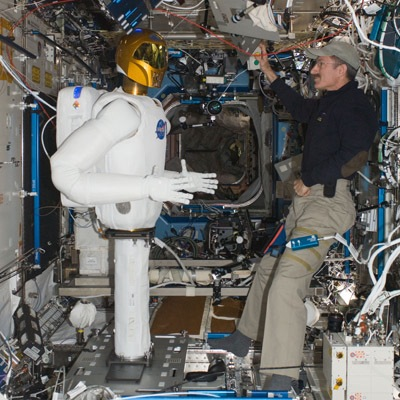
\includegraphics[width=\linewidth]{robot/aerospace.jpg}
        \caption{}
        \label{rob:subfig1}
    \end{subfigure}
    \begin{subfigure}[b]{.23\textwidth}
        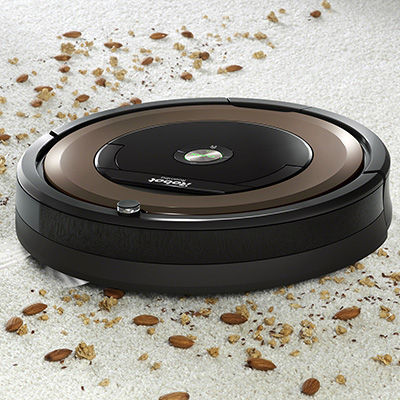
\includegraphics[width=\linewidth]{robot/consumer.jpg}
        \caption{}
        \label{rob:subfig3}
    \end{subfigure}
    \begin{subfigure}[b]{.23\textwidth}
        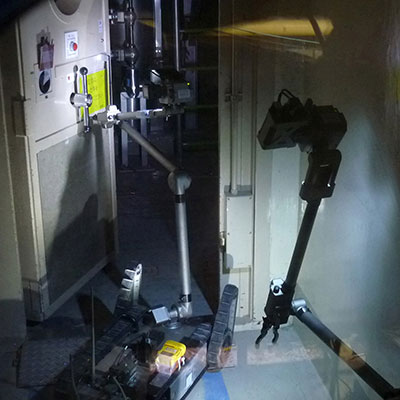
\includegraphics[width=\linewidth]{robot/disasterresponse.jpg}
        \caption{}
        \label{rob:subfig4}
    \end{subfigure}
    \begin{subfigure}[b]{.23\textwidth}
        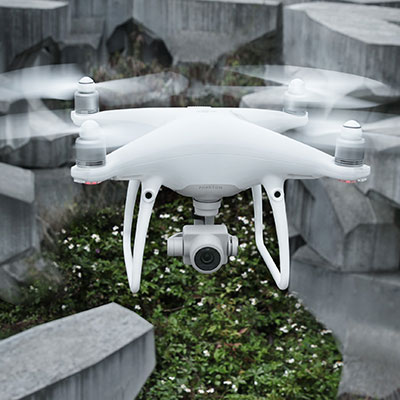
\includegraphics[width=\linewidth]{robot/drones.jpg}
        \caption{}
        \label{rob:subfig5}
    \end{subfigure}
    \begin{subfigure}[b]{.23\textwidth}        
        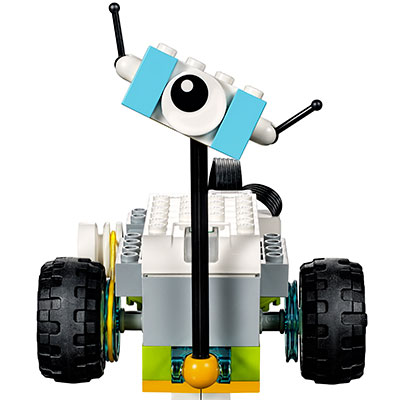
\includegraphics[width=\linewidth]{robot/education.jpg}
        \caption{}
        \label{rob:subfig6}
    \end{subfigure}
    \begin{subfigure}[b]{.23\textwidth}
        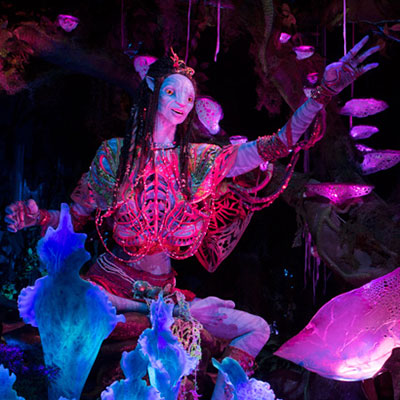
\includegraphics[width=\linewidth]{robot/entertainment.jpg}
        \caption{}
        \label{rob:subfig7}
    \end{subfigure}
    \begin{subfigure}[b]{.23\textwidth}
        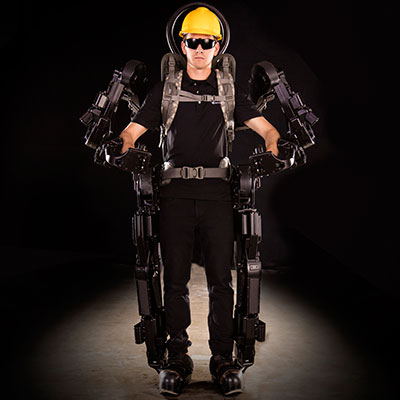
\includegraphics[width=\linewidth]{robot/exoskeleton.jpg}
        \caption{}
        \label{rob:subfig8}
    \end{subfigure}
    \begin{subfigure}[b]{.23\textwidth}
        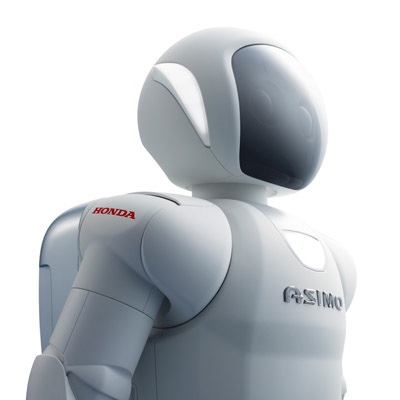
\includegraphics[width=\linewidth]{robot/humanoid.jpg}
        \caption{}
        \label{rob:subfig9}
    \end{subfigure}
    \begin{subfigure}[b]{.23\textwidth}
        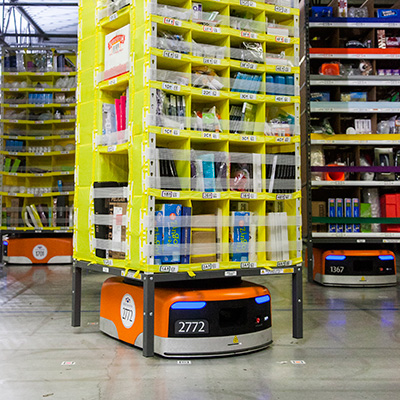
\includegraphics[width=\linewidth]{robot/industrial.jpg}
        \caption{}
        \label{rob:subfig10}
    \end{subfigure}
    \begin{subfigure}[b]{.23\textwidth}
        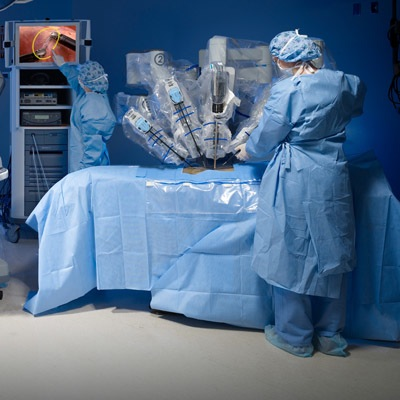
\includegraphics[width=\linewidth]{robot/medical.jpg}
        \caption{}
        \label{rob:subfig11}
    \end{subfigure}
    \begin{subfigure}[b]{.23\textwidth}
        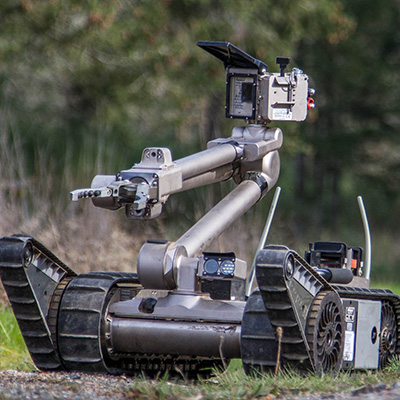
\includegraphics[width=\linewidth]{robot/military.jpg}
        \caption{}
        \label{rob:subfig12}
    \end{subfigure}
    \begin{subfigure}[b]{.23\textwidth}
        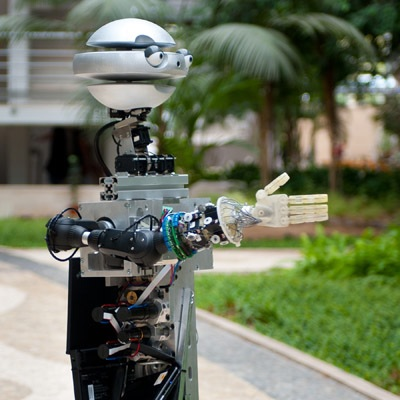
\includegraphics[width=\linewidth]{robot/research.jpg}
        \caption{}
        \label{rob:subfig13}
    \end{subfigure}
    \begin{subfigure}[b]{.23\textwidth}
        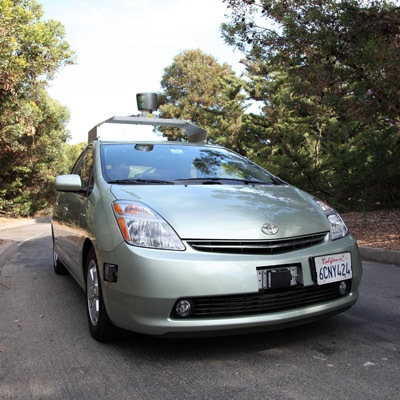
\includegraphics[width=\linewidth]{robot/autonomous.jpg}
        \caption{}
        \label{rob:subfig2}
    \end{subfigure}
    \begin{subfigure}[b]{.23\textwidth}
        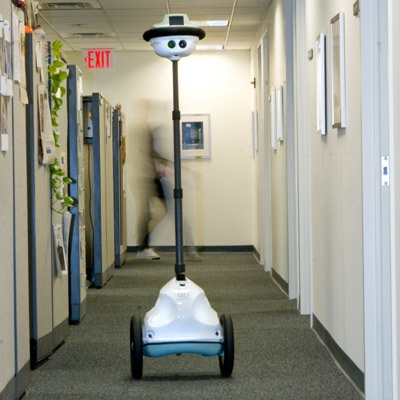
\includegraphics[width=\linewidth]{robot/telepresence.jpg}
        \caption{}
        \label{rob:subfig14}
    \end{subfigure}
    \begin{subfigure}[b]{.23\textwidth}
        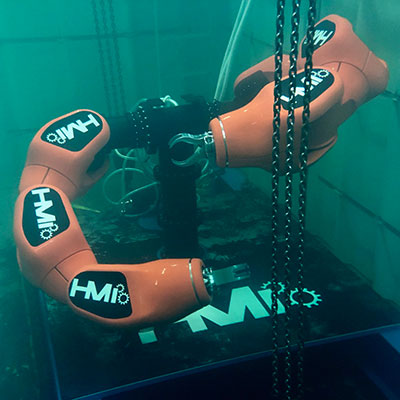
\includegraphics[width=\linewidth]{robot/underwater.jpg}
        \caption{}
        \label{rob:subfig15}
    \end{subfigure}
    \caption{Contoh Jenis-Jenis Robot\cite{b1}.}
    \label{fig:robot_figures}
\end{figure}
Penjelasan mengenai tugas dan fungsi masing-masing jenis robot pada Gambar \ref*{fig:robot_figures} adalah sebagai berikut:
\begin{enumerate}[label=(\alph*)]
    \item \textit{Aerospace}: Kategori \textit{aerospace} mencakup semua jenis robot terbang dan juga robot yang dapat beroperasi di luar angkasa. Pada gambar terlihat robot luar angkasa milik The National Aeronautics and Space Administration (NASA) yang bernama Robonaut. Robot ini memiliki bentuk mirip dengan manusia yang dibuat untuk membantu tugas-tugas astronot di stasiun luar angkasa.
    \item Konsumen: Robot konsumen adalah robot yang dapat dibeli dan digunakan hanya untuk bersenang-senang atau untuk membantu manusia dengan tugas sehari-hari seperti membersihkan ruangan. Gambar menunjukkan salah satu robot yang membantu membersihkan lantai rumah secara otomatis yaitu penyedot debu Roomba.
    \item Tanggap Bencana: Robot-robot ini melakukan pekerjaan berbahaya setelah keadaan darurat. Contoh robot ini tertampil pada gambar yaitu Packbots yang digunakan untuk memeriksa kerusakan di pembangkit listrik tenaga nuklir Fukushima Daiichi setelah gempa bumi dan tsunami melanda Jepang pada tahun 2011.
    \item \textit{Drone}: \textit{Drone} atau disebut kendaraan udara tanpa awak yang digunakan dalam berbagai ukuran untuk menyelesaikan tugas melalui jalur udara. \textit{Drone} memiliki berbagai jenis baling-baling dan ukuran. Gambar menunjukkan \textit{drone} DJI Phantom 4 yang memiliki jenis baling-baling 4 buah atau biasa disebut \textit{drone} \textit{quadcopter}. 
    \item Pendidikan: Kategori robot ini ditujukan untuk generasi peminat robotika berikutnya yang dapat digunakan sebagai bahan pembelajaran di rumah atau di ruang kelas. Robot pada gambar adalah robot Lego WeDo 2.0 yang dapat digunakan sebagai sumber belajar pemrograman pada robot.
    \item Hiburan: Robot-robot ini dirancang untuk membangkitkan respons emosional dan membuat manusia tertawa atau merasa terkejut atau kagum. Salah satu contoh robot hiburan pada gambar adalah Navi Shaman, robot ini milik Disney yang dipasang di taman hiburan mereka. 
    \item \textit{Exoskeleton}: Robot \textit{exoskeleton} adalah robot yang membantu pergerakan tubuh. Robot \textit{exoskeleton} pada gambar adalah robot Ekso yang berfungsi untuk membantu pasien lumpuh. Robot ini juga dapat digunakan untuk rehabilitasi fisik dan untuk memungkinkan pasien yang lumpuh berjalan lagi.
    \item Humanoid: Robot ini menyerupai fisik manusia dan mengerjakan tugas-tugas manusia. Robot humanoid pada gambar adalah robot milik Honda yaitu robot Asimo.
    \item Industri: Robot industri biasanya terdiri dari lengan manipulator yang dirancang untuk melakukan tugas berulang. Kategori ini juga mencakup robot yang bekerja dalam sebuah sistem seperti robot gudang Amazon pada gambar dan robot kolaboratif pada pabrik yang dapat beroperasi bersama pekerja manusia.
    \item Medis: Robot medis dan perawatan kesehatan mencakup sistem seperti robot bedah da Vinci pada gambar, \textit{bionic prostheses} yang menggantikan bagian tertentu fisik manusia, serta \textit{exoskeleton}.
    \item Militer dan Keamanan: Robot yang bekerja pada bidang militer dan keamanan baik untuk membantu manusia maupun menggantikan manusia dalam tugas berbahaya militer dan keamanan. Contoh robot dalam gambar adalah  PackBot dari Endeavor Robotics yang digunakan di Irak dan Afghanistan untuk mencari alat peledak.
    \item Penelitian: Robot yang digunakan duntuk membantu para peneliti melakukan penelitian dan berbagai tugas lainnya. Robot yang ditampilkan pada gambar adalah Flash yang dirancang untuk mengeksplorasi bagaimana manusia merespons sebuah robot yang dapat berbicara, menggerakkan tangan, dan membuat ekspresi wajah.
    \item \textit{Self-Driving Cars}: Robot ini memiliki bentuk kendaraan yang dapat menyetir sendiri secara otomatis. Contoh robot pada gambar yaitu mobil \textit{self-driving} Toyota Prius milik Google. 
    \item \textit{Telepresence}: Robot \textit{telepresence} memiliki kemampuan yang memungkinkan pengguna untuk hadir di suatu tempat tanpa benar-benar pergi ke sana. Contoh robot terlihat pada gambar adalah Anybots QB yang membuat pengguna mampu mengendalikan robot dengan masuk ke avatar robot melalui internet untuk mengendarainya, melihat apa yang dilihatnya, dan berbicara dengan orang-orang sekitarnya.
    \item \textit{Underwater}: Robot yang dibuat khusus untuk beroperasi di bawah air. Terlihat pada gambar yaitu Aquanaut yang dikembangkan Houston Mechatronics yang dapat bertransformasi menjadi kapal selam dan robot setengah humanoid.
\end{enumerate}


\subsection{Robot \textit{Autonomous}}
\label{sec:Robot_Autonomous} 
    
Setiap robot memiliki tingkat otonomi yang berbeda mulai dari robot yang dikendalikan manusia yang melakukan tugas yang dikendalikan sepenuhnya oleh manusia hingga robot yang sepenuhnya \auto\ yang melakukan tugas tanpa perintah eksternal. Robot \auto\ merupakan robot yang mampu memutuskan aksinya untuk mengeksekusi perintah secara mandiri tanpa campur tangan manusia hingga tujuan tercapai\cite{b2}. Robot ini memanfaatkan berbagai sensor untuk memperoleh informasi dan menggunakan hasil pelatihan data untuk memutuskan apa yang akan dilakukan. Robot dapat diklasifikasikan sebagai robot \auto\ jika mereka kemampuan dalam persepsi, pengambilan keputusan dan aksi secara mandiri. Walaupun robot ini tidak memerlukan tenaga manusia saat beroperasi, robot ini masih memerlukan manusia untuk melakukan perawatan secara berkala.

Robot \auto\ saat ini dioperasikan dalam berbagai bidang dalam kehidupan sehari-hari. 
Robot \auto\ biasa digunakan dalam transportasi logistik misal dalam \textit{e-commerce} menggunakan robot \auto\ untuk melakukan transportasi barang, pemenuhan pesanan, penyortiran, dan pengatur penyimpanan. Robot ini juga digunakan untuk mengangkat barang berat dan mengangkut barang ke seluruh ruangan dalam gudang-gudang. 
Robot \auto\ dalam industri umumnya memiliki bagian tambahan khusus seperti lengan dan konveyor untuk memudahkan produksi dan distribusi.
% This also enables instant, accurate, and easily accessible documentation of the process.

\subsection{Robot Bergerak}
\label{sec:Robot_Bergerak}

Robot bergerak merupakan kombinasi dari berbagai macam perangkat keras dan perangkat lunak untuk bergerak di ruang bebas. Robot ini mencakup semua robot yang memiliki kemampuan mobilitas. Robot beroda merupakan bentuk umum yang biasa dijumpai untuk robot bergerak. Gambar \ref*{fig:Ch02_control_scheme} menunjukkan alur kontrol untuk robot beroda. Pertama, robot akan mencari informasi mengenai lingkungan dan mengartikan informasi yang diperoleh. Informasi akan dibuat menjadi peta yang kemudian digunakan untuk menentukan posisi robot dalam peta tersebut atau disebut lokalisasi. Lokalisasi menghasilkan informasi koordinat robot pada ruangan untuk proses selanjutnya yaitu menentukan respon robot sesuai kercerdasan robot (\textit{cognition}). Robot kemudian menentukan jalur yang akan ditempuh selanjutnya dan memberi perintah pada aktuator agar robot bergerak menuju tujuan selanjutnya. 

\begin{figure}[H]
    \centering
    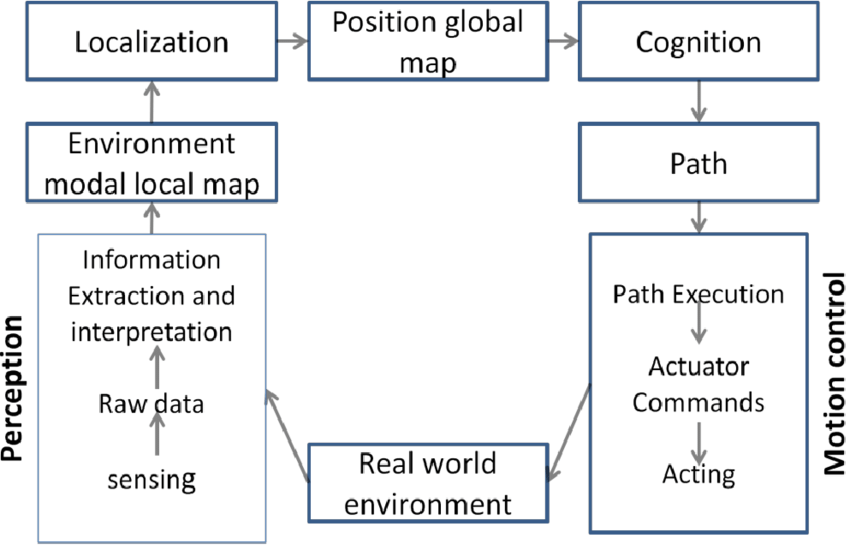
\includegraphics[scale=0.5]{control_scheme.png}
    \caption{Alur Kontrol Robot Beroda \cite{b3}.}
    \label{fig:Ch02_control_scheme}
\end{figure}
% n at: https://www.researchgate.net/publication/267989738

Pada dasarnya, robot bergerak memiliki empat kemampuan dasar yaitu \textit{locomotion, sensing,} kontrol dan komunikasi\cite{b3}. 
\textit{Locomotion} memungkinkan robot bergerak tanpa batas 
di seluruh lingkungannya. 
\textit{Sensing} adalah bagaimana robot mengetahui dan mengukur sifat-sifat dalam dirinya dan lingkungannya.
Kontrol adalah bagaimana robot berpikir untuk menentukan aksi. Komunikasi adalah cara robot mengirim dan menerima pesan dengan robot satu sama lain atau dengan operator. Kemampuan-kemampuan ini memunculkan adanya berbagai macam cara yang robot untuk bergerak dengan pemilihan berbagai macam desain algoritma dan perangkat robot. 

Robot beroda dengan komposisi roda tiga buah merupakan bentuk robot bergerak sederhana yang sering dijumpai pada kehidupan sehari-hari. Gambar \ref*{fig:Ch02_mobile_robot} menunjukkan \textit{base} untuk robot beroda tiga yaitu robot Pioneer 3DX. Roda kanan dan roda kiri adalah sumber gerak robot yang diberi motor robot sedangkan roda \textit{castor} adalah roda penyeimbang robot. Robot bergerak dapat dimodelkan menjadi \textit{physical model} dari badan dan komponen robot seperti pengatur kecepatan, motor, \textit{gearbox}, dsb. 

% Second approach is based on experimental fitting of recorded mobile robot velocity data regarding reference velocity data. 
\begin{figure}[H]
    \centering
    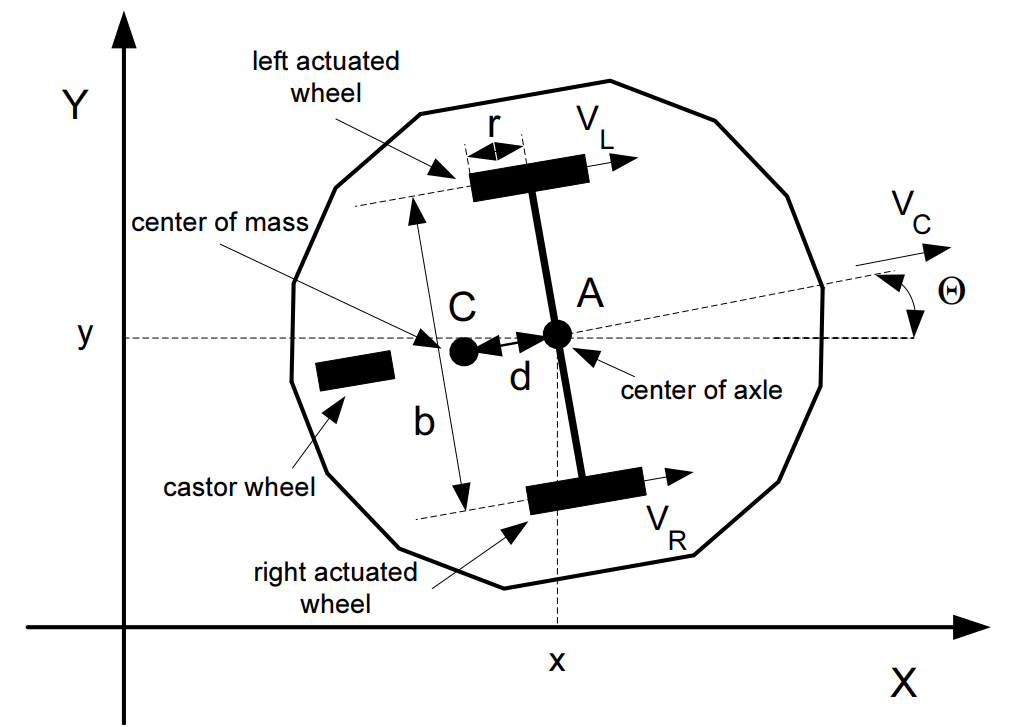
\includegraphics[scale=0.5]{mobile_robot.png}
    \caption{Geometri Robot Pioneer 3DX \cite{b4}.}
    \label{fig:Ch02_mobile_robot}
\end{figure}
% https://www.researchgate.net/publication/228561343_Modelling_of_Mobile_Robot_Dynamics

Gerak lurus robot diproduksi dengan menggerakkan roda kanan dan roda kiri secara bersamaan, sedangkan untuk belok kanan yaitu dengan menaikkan kecepatan roda kiri lebih tinggi dari roda kanan dan sebaliknya untuk belok kiri. Robot ini dapat berputar di tempat dengan menggerakkan satu roda ke depan dan satu ke belakang dari roda kanan dan roda kiri. Roda dilengkapi dengan \textit{encoder} dan sensor pembaca kecepatan untuk mencatat pergerakan robot. Gambar juga menunjukkan komponen-komponen geometri robot antara lain yaitu $r$ sebagai jari-jari roda robot $(mm)$, $v_L$ dan $v_R$ sebagai kecepatan roda kanan dan roda kiri $(mm/s)$, $x$ dan $y$ yang mewakilkan posisi pada koordinat kartesian dalam $(mm)$, dan $b$ adalah jarak antar roda penggerak dalam $(mm)$. Persamaan gerak dinamis robot beroda tiga dapat diturunkan menggunakan formula Euler-Lagrange\cite{b4} pada persamaan \ref*{eq:aeuler_lagrange}:
\begin{equation}
    \glsadd{diferensial_biasa}\glsadd{diferensial_p}
    \diff{}{t}\left(\diffp{L}{\dot{q}_i}\right)-\frac{L}{q_i}=Q_i
    \label{eq:aeuler_lagrange}
\end{equation}
\begin{tabbing}
    dengan: \=\\
        \>$L$ \qquad \=: perbedaan energi kinetik $(T)$ dan energi potensial $(U)$,\\ 
        \>$q_i$ \>: koordinat umum $\bar{x}=\frac{1}{N}\sum_{i=1}^n x_i$,\\
        \>$Q_i$ \>: gaya yang bekerja pada sistem mekanik.
\end{tabbing}
Robot diasumsikan hanya bergerak pada permukaan datar sehingga energi potensial robot adalah nol $(U = 0)$. Persamaan \ref*{eq:aeuler_lagrange} dapat ditulis ulang menjadi persamaan \ref*{eq:euler_lagrange2a} dan persamaan \ref*{eq:euler_lagrange2b}.
\begin{align}
    \label{eq:euler_lagrange2a}
    \glsadd{diferensial_biasa}\diff{}{t}\left(\glsadd{diferensial_p}\diffp{L}{\dot{\Theta}_R}\right)-\glsadd{diferensial_p}\diffp{L}{\Theta_R}=M_R-K\dot{\Theta}_R,\\
    \label{eq:euler_lagrange2b}
    \diff{}{t}\left(\glsadd{diferensial_p}\diffp{L}{\dot{\Theta}_L}\right)-\glsadd{diferensial_p}\diffp{L}{\Theta_L}=M_L-K\dot{\Theta}_L.
\end{align}
\begin{tabbing}
dengan: \=\\
        \>$\Theta_R$ \qquad \=: posisi sudut roda kanan $(rad)$,\\ 
        \>$\Theta_L$ \qquad \>: posisi sudut kiri $(rad)$,\\
        \>$\dot{\Theta}_R$ \>: kecepatan angular roda kanan $(rad/s)$,\\
        \>$\dot{\Theta}_L$ \>: kecepatan angular roda kiri $(rad/s)$,\\
        \>$M_R$ \>: torsi roda kanan $(kgmm/s^2)$,\\
        \>$M_L$ \>: torsi roda kiri $(kgmm/s^2)$,\\
        \>$K\dot{\Theta}_R$ \>: nilai gaya gesek viskos roda kanan $(kgmm/s^2)$,\\
        \>$K\dot{\Theta}_L$ \>: nilai gaya gesek viskos roda kiri $(kgmm/s^2)$,\\
        \>$Q_i$ \>: gaya yang bekerja pada sistem mekanik.
\end{tabbing}
kemudian kedua persamaan di atas dapat ditulis ulang menjadi:
\begin{align}
    \label{eql: 1}
    A\ddot{\Theta}_R+B\ddot{\Theta}_L=M_R-K\dot{\Theta}_R,\\
    \label{eql: 2}
    B\ddot{\Theta}_R+A\ddot{\Theta}_L=M_L-K\dot{\Theta}_L.
\end{align}
Persamaan \ref*{eql: 1} dan \ref*{eql: 2} jika dihubungkan dengan variabel-variabel robot beroda pada Gambar \ref*{fig:Ch02_mobile_robot} akan menghasilkan dua persamaan akhir yaitu:
\begin{align}
    \label{eql: 1a}
    A=\left(\frac{mr^2}{4}+\frac{(I_A+md^2)r^2}{b^2}+I_0\right),\\
    \label{eql: 1b}
    B=\left(\frac{mr^2}{4}-\frac{(I_A+md^2)r^2}{b^2}\right),
\end{align}
\begin{tabbing}
    dengan: \=\\
        \>$m$ \qquad \=: massa seluruh robot $(kg)$,\\ 
        \>$I_A$ \>: momen inersia seluruh robot terhadap titik A $(kgmm^2)$,\\
        \>$I_0$ \>: momen inersia gabungan motor penggerak (rotor) dan roda $(kgmm^2)$.
\end{tabbing}

% Mobile Robot Control on a Reference Path/ https://www.researchgate.net/publication/224616884_Mobile_Robot_Control_on_a_Reference_Path : ngga dipakai

\section{Sensor Persepsi}
\label{sec:sensor}  
    Sensor persepsi adalah sensor yang digunakan untuk mendeteksi dan mengenali objek-objek di sekitar.
    Ada berbagai sensor yang dapat digunakan robot untuk membaca dan memetakan lingkungan sekitar tanpa memerlukan kontak fisik. Sensor-sensor ini dapat bekerja untuk menentukan jarak objek di sekitarnya hingga dapat memberi gambaran bentuk objek target. Jenis sensor robot dapat dibedakan menjadi dua yaitu sensor \textit{proprioceptive} dan sensor \textit{exteroceptive}\cite{b5}. Sensor \textit{proprioceptive} mengukur nilai-nilai internal sistem (robot) seperti kecepatan motor, beban roda, sudut lengan robot, tegangan baterai, dsb. Sensor \textit{exteroceptive} digunakan untuk memperoleh informasi dari lingkungan robot seperti pengukuran jarak, intensitas cahaya, amplitudo suara, dsb. Pada subbab ini akan dijelaskan beberapa contoh sensor persepsi \textit{exteroceptive} yang dapat digunakan untuk mendeteksi posisi objek-objek sekitar robot.
%    https://www.globalspec.com/reference/8277/348308/Chapter-6-Classification-of-Sensors
   
   \subsection{Kamera RGB-D}
    \label{subsec:Sub-Metode_Kamera}
    
    Robot \auto\ biasanya memiliki beberapa kemampuan seperti \textit{Obstacle Avoidance (OA), Augmented Reality (AR), Simultaneous Localization and Mapping (SLAM),} dan \textit{Mobile Object Tracking (MOT)} yang semuanya membutuhkan informasi akurat mengenai posisi objek sekitarnya. Pendeteksian objek menggunakan kamera yang biasanya dapat mengetahui jarak target untuk memperoleh informasi lengkap seperti letak dan tekstur target. Kamera yang memiliki kemampuan tersebut disebut dengan kamera RGB-D (\textit{Red, Green, and Blue - Depth}). Kamera RGB-D memberikan informasi berupa gabungan visual warna, bentuk dan kedalaman untuk mengenali target\cite{b6}. Contoh hasil bacaan kamera RGB-D diperlihatkan pada Gambar \ref{fig:Ch02_rgbd_kamera}.
    \begin{figure}[H]
        \centering
        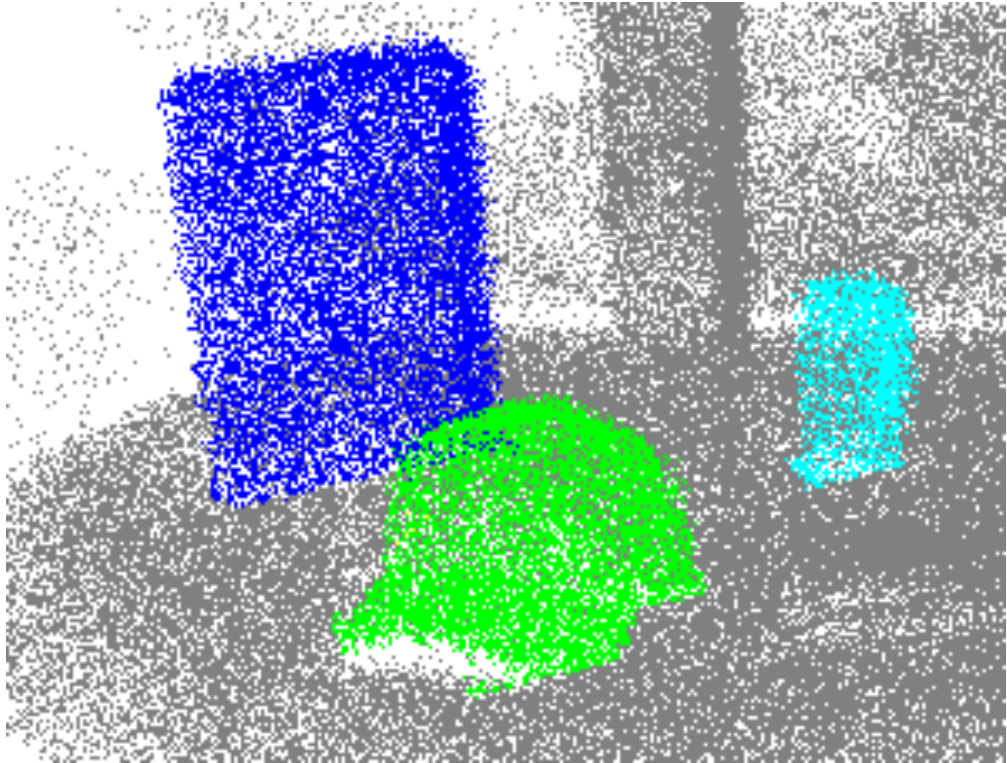
\includegraphics[scale=0.3]{rgbd.png}
        \caption{Contoh hasil bacaan kamera RGB-D\cite{b6}.}
        \label{fig:Ch02_rgbd_kamera}
    \end{figure}

    % https://www.researchgate.net/publication/336829539_RGB-D_Image_Analysis_and_Processing : sumber utamaaaaaaaaaaaa bab di bawah
    \subsubsection{Jenis-jenis Kamera RGB-D}
    \label{subsec: jenis_rgb_d}
    Kamera yang digunakan secara aktif memodifikasi \textit{scene} untuk menyederhanakan masalah rekonstruksi dapat dimasukkan dalam sensor aktif. Ada dua jenis kelas kamera sensor aktif  yang didasarkan pada prinsip kerja yang berbeda, yang disebut kamera \textit{Time of Flight} (ToF) dan \textit{Structured Light} (SL)\cite{b7}.
    % Sarbolandi H, Lefloch D, Kolb A (2015) Kinect range sensing: structured-light versus time of-flight kinect. Comput Vis Image Underst 139:1–20. https://doi.org/10.1016/j.cviu.2015.05.006
    Kamera SL memproyeksikan pola unik ke dalam \textit{scene} untuk menambahkan fitur tambahan untuk menyederhanakan pencocokan fitur dan perhitungan kedalaman (\textit{depth}). Tantangan yang dihadapi pendekatan rekonstruksi ini adalah ketika ada wilayah tanpa fitur pada \textit{scene}. Sementara itu, kamera ToF bekerja dengan  memancarkan pulsa cahaya (dapat yang sudah termodulasi) dan mengukur waktu perjalanan pulang pergi pulsa atau pergeseran fase. Sensor moderen untuk kedua kasus tersebut biasanya bekerja dalam domain inframerah (IR) agar tidak mengganggu penglihatan manusia dan memungkinkan penangkapan penampilan pemandangan secara simultan.

    \paragraph{Kamera \textit{Time of Flight}}
    \label{subsec: kamera_tof}
    Prinsip kerja dasar kamera ToF didasarkan pada pengukuran waktu pulsa cahaya yang dipancarkan hingga dipantulkan kembali\cite{b8}.
    % Foix S, Alenya G, Torras C (2011) Lock-in time-of-flight (ToF) cameras: a survey. IEEE Sens J 11(9):1917–1926. https://doi.org/10.1109/JSEN.2010.2101060
    Ada dua jenis kamera TOf. Jenis pertama yaitu kamera \textit{Pulsed Time-of-Flight}, mengukur waktu perjalanan pulang pergi(\textit{round trip time}) dari pulsa cahaya yang dihitung dari kecepatan \textit{shutters} dan kecepatan \textit{clock}. Jarak perjalanan pulang pergi dapat dihitung dengan mengukur keterlambatan antara pengiriman dan penerimaan pulsa cahaya. \textit{Scene depth} dapat dihitung sebagai setengah dari jarak perjalanan pulang pergi yang diukur yaitu:
    \begin{equation}
        \textit{Depth} = \frac{\textit{Speed\ of\ Light}\times \textit{Round\ Trip\ Time}}{2}.
    \end{equation}
    Jenis kedua kamera ToF menggunakan pulsa cahaya yang termodulasi waktu kemudian mengukur pergeseran fase antara pulsa yang dipancarkan dan yang kembali. Pulsa cahaya biasanya dimodulasi oleh gelombang kontinu. Detektor fase digunakan untuk memperkirakan fase pulsa cahaya yang kembali. Setelah itu, \textit{scene depth} diperoleh dengan korelasi antara pergeseran fase dan \textit{scene depth}. Teknik multi-frekuensi dapat digunakan untuk lebih meningkatkan akurasi pengukuran kedalaman yang diperoleh dan rentang pengindraan efektif kamera. Contoh kamera ToF jenis ini adalah Microsoft Kinect One dan Creative Senz3D.

    \paragraph{Kamera \textit{Structured Light}}
    \label{subsec: kamera_sl}
    Jenis kamera SL memiliki cara kerja mirip dengan rekonstruksi stereo yaitu didasarkan pada triangulasi. Konsepnya adalah mengganti salah satu dari dua kamera dalam sistem stereo dengan proyektor. Proyektor dapat diartikan sebagai kamera terbalik. Proyeksi pola terstruktur unik yang diketahui [14] ke dalam \textit{scene} menyebabkan fitur buatan tambahan diperkenalkan ke dalam \textit{scene}. Beberapa sensor (seperti Microsoft Kinect) memproyeksikan pola titik unik [4] dan beberapa sensor lain memproyeksikan urutan temporal garis-garis hitam dan putih. Kamera SL tersebar luas dan sering digunakan dalam penelitian. Sensor komoditas dari kategori ini biasanya bekerja di domain inframerah untuk tidak mengganggu penglihatan manusia dan memungkinkan penangkapan simultan dari gambar warna tambahan. Contoh sensor komoditas berbasis teknologi ini adalah Microsoft Kinect, Primesense Carmine, Asus Xtion Pro, dan Intel Realsense.

    \subsubsection{\textit{Missing Depth}}
    \label{subsec:missing_depth}
    
    Saat ini ada banyak tantangan dalam mengestimasi \textit{scene depth} yang merupakan salah satu bagian mendasar dari setiap sistem penglihatan 3D yang berfokus pada gambar RGB-D.
    Pendekatan \textit{depth-sensing} yang berbeda dapat menyebabkan berbagai masalah dalam kedalaman pemandangan yang diperoleh, sehingga proses penyelesaian dan penyempurnaan \textit{depth} merupakan langkah penting pada langkah pasca-pemrosesan.
    \begin{figure}[H]
        \centering
        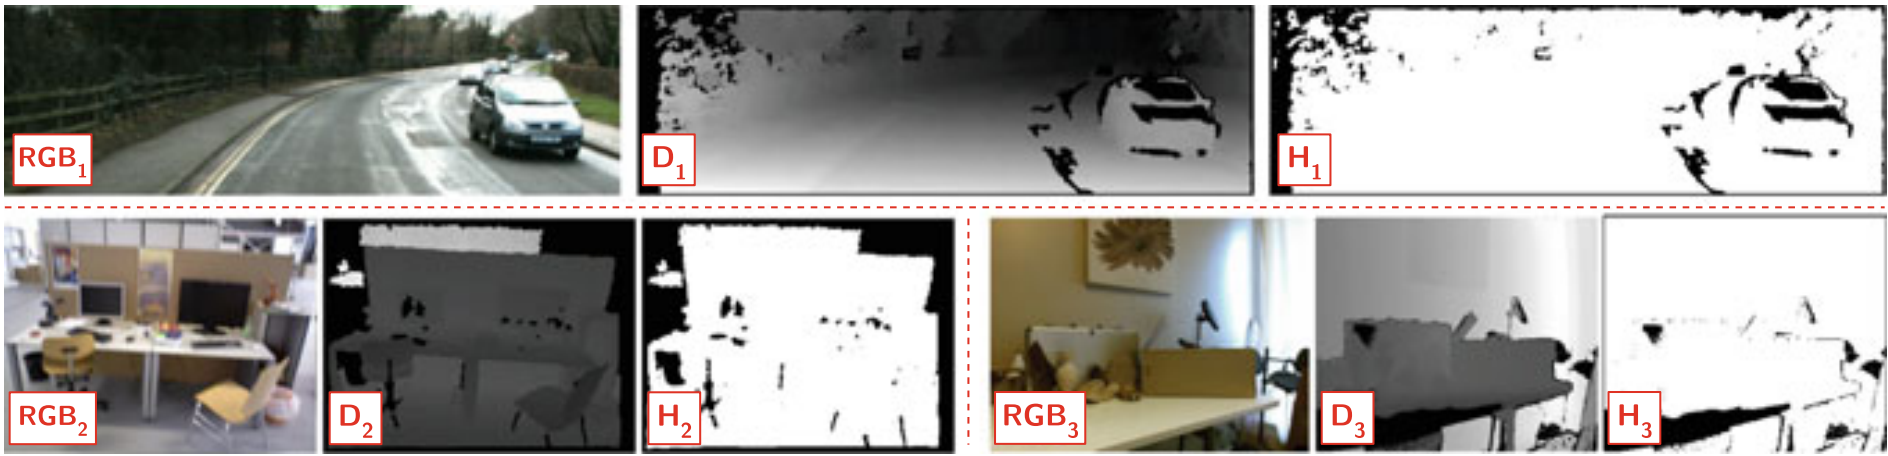
\includegraphics[width=\textwidth]{missing_depth.png}
        \caption{Kedalaman yang Hilang pada Kamera RGB-D\cite{b9}.}
        \label{fig:Ch02_missing_depth}
    \end{figure}

Selain itu, nilai yang hilang kebanyakan berada di \textit{scene} yang berisi wilayah yang tersumbat (kelompok piksel yang terlihat dalam satu gambar tetapi tidak di gambar lain), permukaan tanpa fitur, informasi yang jarang untuk objek pemandangan seperti semak belukar, batas objek yang tidak jelas, objek yang sangat jauh dan sejenisnya. Masalah tersebut dapat dilihat pada Gambar \ref{fig:Ch02_missing_depth}, topeng biner menandai letak nilai \textit{depth} atau kedalaman yang hilang berada dalam disparitas gambar yang dihitung melalui algoritma korespondensi stereo\cite{b9}.  

Perangkat konsumen seperti kamera SL dan kamera ToF adalah sensor \textit{range} aktif yang banyak digunakan untuk berbagai keperluan karena biayanya yang rendah dan ketersediaan yang luas di pasar komersial dengan pengaturan kalibrasi pabrik.
% Additionally, missing values are prevalent in sections of the scene that contain occluded regions ( groups of pixels that are seen in one image but not the other), featureless surfaces, sparse information for a scene object such as shrubbery, unclear object boundaries, very distant objects and alike. 
% Such issues can be seen in Fig. 2.1 (top), wherein the binary mask marks where the missing depth values are in a disparity image calculated via a stereo correspondence algorithm [65]. On the other hand, consumer devices such as structured light and time-of-flight cameras are active range sensors that are more widely utilized for a variety of purposes due to their low cost and wide availability in the commercial market with factory calibration settings [14, 23, 46].
Namun, karena sejumlah kekurangan seperti gangguan iluminasi eksternal, saturasi cahaya sekitar, deteksi pola cahaya yang tidak akurat dengan adanya gerakan dan \textit{error} jalur cahaya aktif yang disebabkan oleh permukaan reflektif atau oklusi, perangkat SL dapat menghasilkan \textit{depth} yang hilang atau nilai \textit{noise} yang paling baik ditangani dengan penghapusan dan pengisian.
% However, due to a number of shortcomings such as external illumination interference [23], ambient light saturation [46], inaccurate light pattern detection in the presence of motion [125] and active light path error caused by reflective surfaces or occlusion [126], consumer structured light devices can result in missing depth or noisy values that are best handled by removal and subsequent filling.
%
% 2.3.1 RGB Image Inpainting 
\paragraph{RGB Image Inpainting}
\label{paragraf: rgb_inpainting}

\textit{Inpainting} atau pengecatan berkaitan dengan penyelesaian masalah pada wilayah target dalam gambar yang muncul akibat dari penghapusan bagian tertentu dari \textit{scene}. Pendekatan awal \textit{inpainting} adalah berusaha untuk secara mulus menyebarkan isofop (garis dalam gambar dengan nilai intensitas yang sama) ke dalam area target ini.
% Inpainting deals with the issue of a plausibly completing a target region within the image often created as a result of removing a certain portion of the scene. Early image inpainting approaches attempted to smoothly propagate the isophotes (lines within the 
Namun, sebagian besar pendekatan pengecatan gambar cenderung mengabaikan aspek penting yang signifikan bagi rasa masuk akal pengamat yang merupakan komponen spasial frekuensi tinggi dari gambar atau tekstur.
Akibatnya, teknik \textit{inpainting} mulai memasukkan ide-ide dari bidang sintesis tekstur (dimana tujuannya adalah untuk menghasilkan wilayah tekstur besar dari sampel tekstur yang lebih kecil tanpa artefak pengulangan yang terlihat di wilayah yang lebih besar) ke dalam proses \textit{inpainting} untuk mengimbangi kurangnya tekstur yang biasa ditemukan di wilayah target setelah selesai.
% However, most of these approaches [15, 133] tend to ignore an important aspect significant to an observer's sense of plausibility, which is the high-frequency spatial component of the image or texture. 

    \begin{figure}[H]
        \centering
        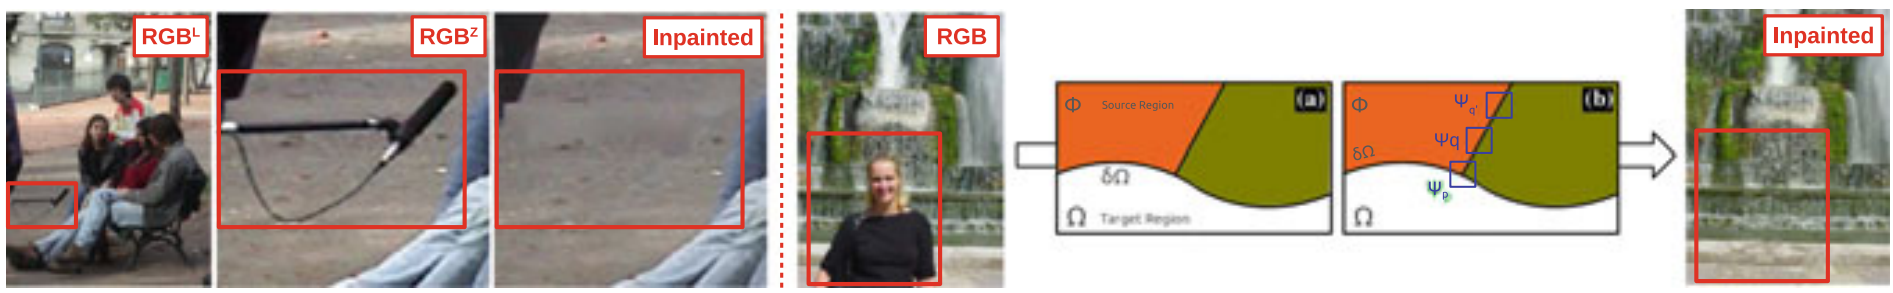
\includegraphics[width=\textwidth]{inpainting.png}
        \caption{Hasil \textit{Inpainting} pada Kamera RGB-D\cite{b9}.}
        \label{fig:Ch02_inpainting}
    \end{figure}


Metode tradisional sintesis tekstur berbasis exemplar diterapkan dengan memprioritaskan urutan pengisian berdasarkan kekuatan gradien di sepanjang batas wilayah target\cite{b10}. 
% In one such approach, the authors of [36] follow traditional exemplar-based texture synthesis methods [43] by prioritizing the order of filling based on the strength of the gradient along the target region boundary. Although the authors of [36] are not the first to carry out inpainting via exemplar-based synthesis [16], previous approaches are all lacking in either structure propagation or defining a suitable filling order that could prevent the introduction of blurring or distortion in shapes and structures. 
Metode berbasis exemplar ini tidak hanya mampu menangani tekstur dua dimensi tetapi juga dapat secara masuk akal menyebarkan struktur linier di dalam gambar. Contoh hasil metode ini dapat dilihat pada Gambar \ref*{fig:Ch02_inpainting}, dimana tekstur air telah disintesis secara masuk akal setelah orang tersebut dikeluarkan dari gambar. Gambar sebelah kiri menunjukkan hasil mikrofon bagian depan telah dihapus dan dicat, tetapi teksturnya tidak akurat dan menyebabkan persepsi kabur. Gambar kanan menunjukkan contoh hasil dan proses pengecatan berbasis exemplar.
Namun, pendekatan ini tidak dapat mengatasi struktur melengkung dan sangat tergantung pada keberadaan lingkungan piksel serupa di wilayah yang dikenal untuk penyelesaian yang masuk akal sehingga beberapa pendekatan lain juga dikembangkan untuk teknik \textit{inpainting}.
% This exemplar-based method [36] is not only capable of handling two-dimensional texture but can plausibly propagate linear structures within the image. An example of the results of this method can be seen in Fig. 2.2 (right), in which water texture has been plausibly synthesized after the person is removed from the image. However, this approach cannot cope with curved structures and is heavily dependent on the existence of similar pixel neighbourhoods in the known region for plausible completion.

% 2.3.2 Depth Filling
\paragraph{\textit{Depth Filling}}
\label{paragraf: depth_filling}

Berbagai teknik \textit{depth filling} yang memanfaatkan teknik-teknik pendekatan \textit{inpainting} juga akan meninggalkan bekasnya pada bagian \textit{depth filling}. Misalnya, penghapusan objek dan \textit{depth filling} gambar RGB-D dilakukan dengan menguraikan gambar menjadi komponen frekuensi spasial tinggi dan rendah yang terpisah melalui filter Butterworth di Fourier Space.
% Nevertheless, just as various depth completion techniques take advantage of other \textit{inpainting} approaches such as [133], with or without modifications [100, 144, 154], exemplar-based image inpainting has also left its mark on depth completion. For instance, in [7], object removal and depth completion of RGB-D images is carried out by decomposing the image into separate high and low spatial frequency components by means of Butterworth filtering in Fourier space. 
Setelah adanya keterikatan gambar frekuensi tinggi dan rendah, informasi frekuensi tinggi (batas objek dan relief tekstur) diisi menggunakan metode sintesis tekstur klasik yang dirumuskan ulang sebagai pendekatan \textit{inpainting} berbasis exemplar piksel demi piksel dan ditingkatkan dengan cara perluasan kueri dalam ruang pencarian, kemudian komponen frekuensi rendah (geometri bentuk yang mendasarinya) diselesaikan melalui \textit{inpainting} berbasis exemplar. Hasilnya  digabungkan kembali dalam domain frekuensi untuk menghasilkan hasil akhir. Hasil dapat dilihat pada Gambar \ref*{fig:Ch02_depth_filling} bahwa gambar yang dihasilkan tajam dan tanpa artefak tambahan. Objek telah dihapus dari gambar RGB-D dan nilai kedalaman yang hilang dalam gambar telah diisi.
% After the disentanglement of high and low frequency images, the high-frequency information (object boundaries and texture relief) is filled using a classic texture synthesis method [43] reformulated as a pixel-by-pixel exemplar-based inpainting approach and enhanced by means of query expansion within the search space, and the low frequency component (underlying shape geometry) is completed via [2]. The results are then recombined in the frequency domain to generate the final output. As can be seen in Fig. 2.5, the produced images are sharp and with no additional artefacts.
\begin{figure}[H]
    \centering
    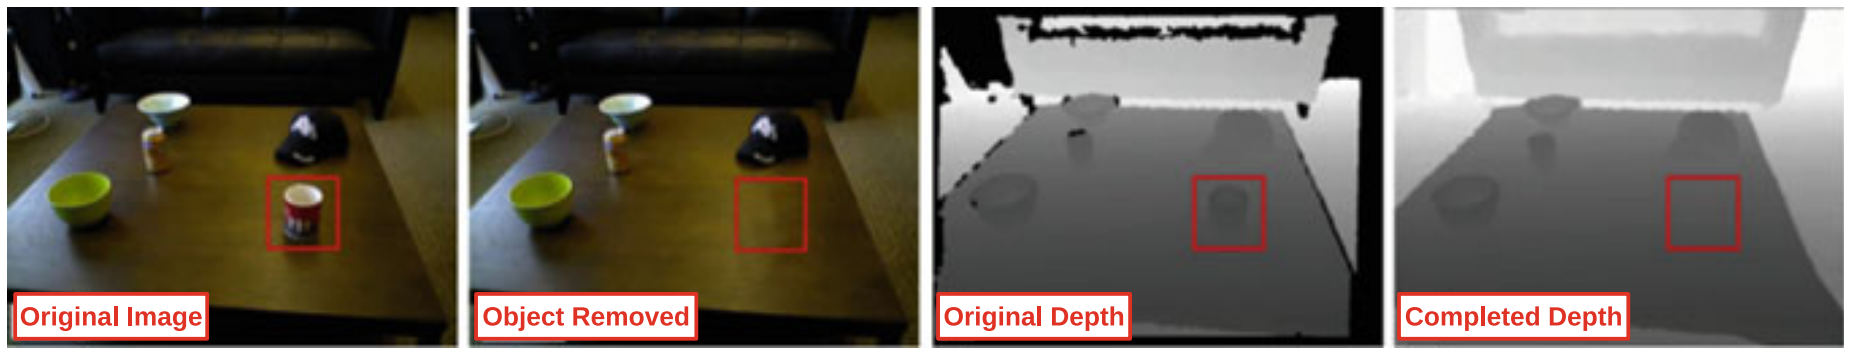
\includegraphics[width=\textwidth]{depth_filling.png}
    \caption{Contoh Hasil \textit{Depth Filling}\cite{b9}.}
    \label{fig:Ch02_depth_filling}
\end{figure}

% Pekerjaan dalam [5] mengembangkan teknik pengecatan RGB dari [36] untuk menciptakan pendekatan berbasis exemplar yang secara eksplisit dirancang untuk melengkapi gambar kedalaman. Ini dicapai dengan menambahkan syarat khusus yang berfokus pada karakteristik gambar kedalaman ke dalam fungsi prioritas untuk menentukan tambalan mana yang diutamakan dalam urutan pengisian. Adanya syarat tekstur dan batas membuat relief permukaan dan tekstur terpelihara dengan baik dalam gambar kedalaman setelah selesai sehingga mengarah ke hasil yang lebih masuk akal dengan artefak yang lebih sedikit. Seperti yang dapat dilihat pada Gambar 2.6, teknik penyelesaian RGB [36] yang diterapkan pada gambar kedalaman menghasilkan banyak artefak yang tidak diinginkan dapat [5] menghasilkan output kedalaman yang lebih tajam.
% The work in [5] extends on the seminal RGB inpainting technique of [36] to create an exemplar-based approach explicitly designed to complete depth images. This is achieved by adding specific terms focusing on the characteristics of depth images into the priority function, which determines which \textit{patch}es take precedence in the filling order. By introducing texture and boundary terms, the authors of [5] ensure that surface relief and texture are well preserved in the depth image after completion, leading to more plausible results with fewer artefacts. As can be seen in Fig. 2.6, the RGB completion technique [36] applied to depth images produces many undesirable artefacts while [5] generates sharper depth outputs.
Pemecahan masalah pengisian kedalaman menggunakan kerangka kerja berbasis exemplar masih memiliki banyak tantangan yang harus dihadapi oleh proses penyelesaian.  Salah satunya jika kedalaman pemandangan bukan dari tampilan \textit{fronto-parallel} maka tidak ada jaminan bahwa nilai kedalaman yang benar dapat diprediksi untuk wilayah yang hilang melalui pengambilan sampel \textit{patch} ketika mencoba menemukan \textit{patch} serupa.
% Even though solving the depth filling problem using an exemplar-based framework has the potential to produce outputs in which structural continuity within the scene is preserved and granular relief texture is accurately and consistently replicated in the missing depth regions, there are still many challenges the completion process must contend with. For instance, if the scene depth is not of a fronto-parallel view, there is no guarantee that correct depth values can be predicted for the missing regions via \textit{patch} sampling even if the \textit{patch}es undergo different transformations such as rotation, scale, shear, aspect ratio, keystone corrections, gain and bias colour adjustments, and other photometric transformations in the search space when trying to find similar \textit{patch}es to sample from [4].
Cara untuk mengatasi masalah ini yaitu dengan penyelesaian matriks yang baru-baru ini muncul sebagai formulasi masalah penyelesaian gambar, terutama setelah diamati bahwa tambalan serupa dalam gambar RGB-D terletak pada subruang dimensi rendah dan dapat diperkirakan oleh matriks dengan peringkat rendah\cite{b11}. Pendekatan dengan matriks menyajikan metode aljabar linier untuk peningkatan gambar kedalaman berbasis penyelesaian matriks peringkat rendah untuk secara bersamaan menghilangkan \textit{noise} dan menyelesaikan gambar kedalaman menggunakan gambar RGB yang sesuai. 

\begin{figure}[H]
    \centering
    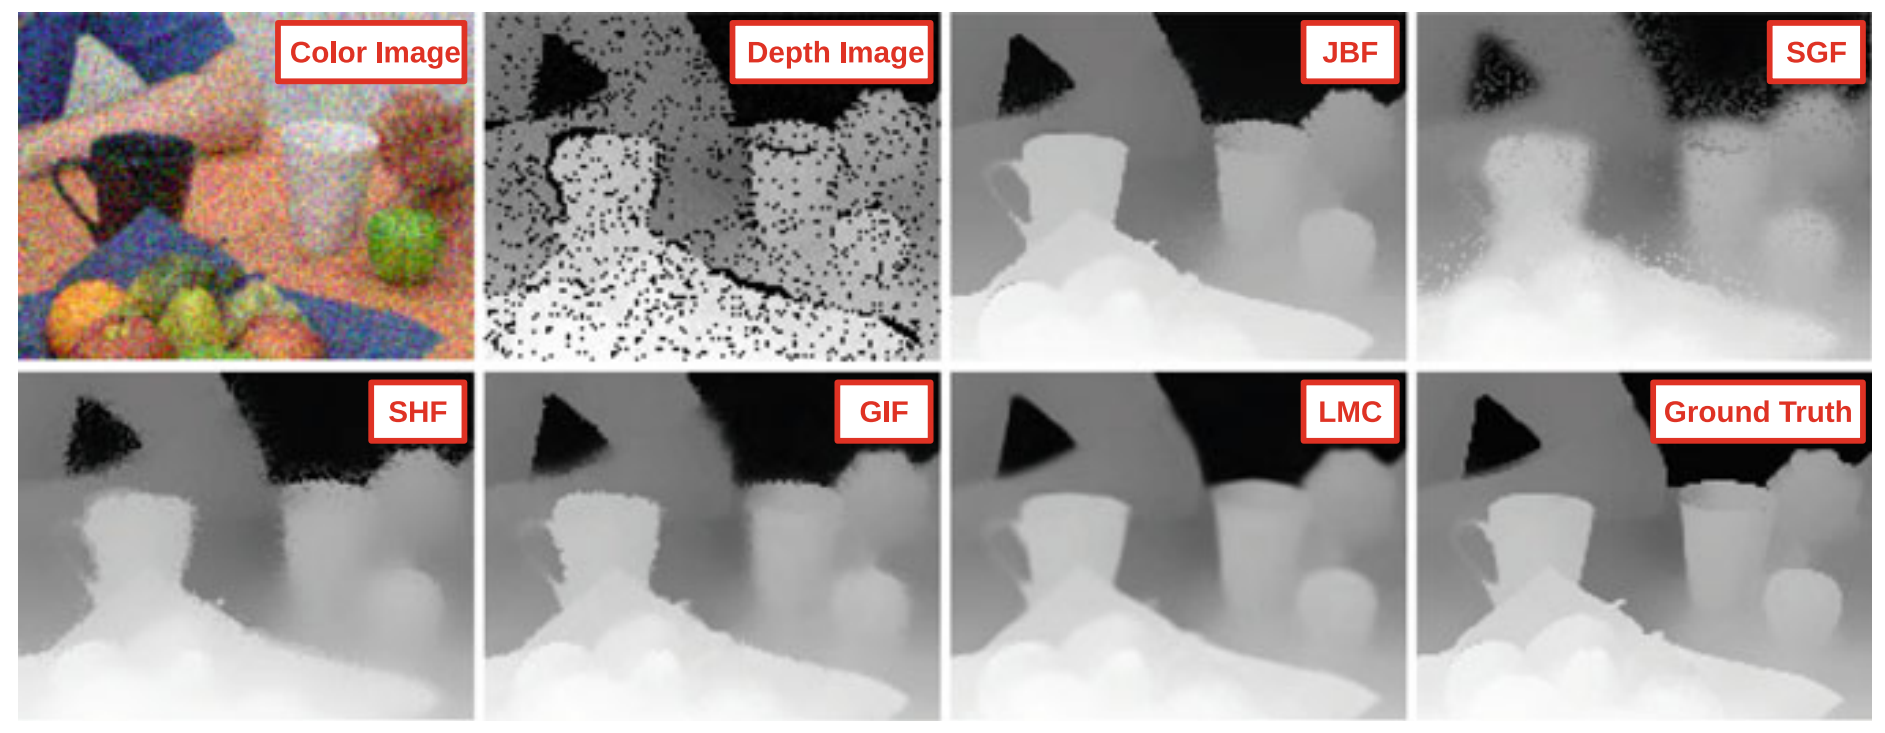
\includegraphics[width=\textwidth]{filling_matriks.png}
    \caption{Contoh Hasil \textit{Depth Filling} Pendekatan Matriks\cite{b9}.}
    \label{fig:Ch02_filling_matriks}
\end{figure}

\textit{De-noising} dan penyelesaian simultan dicapai dengan batasan subruang peringkat rendah yang diberlakukan pada matriks dengan \textit{patch} RGB-D melalui faktorisasi yang tidak lengkap akan
% To combat some of these issues, matrix completion has recently emerged as an interesting formulation of the image completion problem, especially since it has been observed [104] that similar \textit{patch}es in an RGB-D image lie in a low-dimensional subspace and can be approximated by a matrix with a low rank. The approach in [104] presents a linear algebraic method for low-rank matrix completion-based depth image enhancement to simultaneously remove noise and complete depth images using the corresponding RGB images, even if they contain heavily visible noise. In order to accomplish simultaneous de-noising and completion, the low-rank subspace constraint is enforced on a matrix with RGB-D \textit{patch}es via incomplete factorization
menghasilkan penangkapan struktur gambar yang berpotensi bergantung pada pemandangan, baik dari kedalaman maupun ruang warna. Peringkat berbeda dari \textit{patch} ke \textit{patch} tergantung pada struktur gambar, sehingga metode diusulkan untuk secara otomatis memperkirakan nomor peringkat berdasarkan data. Gambar \ref*{fig:Ch02_filling_matriks} menunjukkan kemampuan kinerja pendekatan ini dibandingkan dengan metode penyelesaian kedalaman lainnya seperti \textit{joint bilateral filtering} (JBF), \textit{structure-guided fusion} (SGF), \textit{spatio-temporal hole filling} (SHF) dan \textit{guided inpainting and filtering} (GIF). Pendekatan ini menghasilkan hasil yang bagus walaupun dari input gambar RGB mengandung banyak \textit{noise}.
% which results in capturing the potentially scene-dependent image structures both in the depth and colour space. The rank differs from \textit{patch} to \textit{patch} depending on the image structures, so a method is proposed to automatically estimate a rank number based on the data. Figure 2.7 demonstrates the performance capabilities of this approach compared to other depth completion methods, such as joint bilateral filtering (JBF) [122], structure-guided fusion (SGF) [120], spatio-temporal hole filling (SHF) [25] and guided inpainting and filtering (GIF) [100]. This approach [104] generates particularly impressive results in that the input RGB image is very noisy (Fig. 2.7—Colour Image). Before the comparisons, a de-noising method [37] is applied to the noisy RGB image used as an input for the comparators

 
    \subsection{Sensor Ultrasonik}
    \label{subsec:Ultrasonik}
    Sensor ini memancarkan gelombang ultrasonik untuk mengukur jarak dengan target. Sensor akan menghitung waktu antara pancaran dengan pantulan untuk menghitung jarak. Sinyal ultrasonik memiliki kisaran frekuensi 30 kHz hingga 5 MHz yang dapat digunakan untuk menghasilkan pulsa. Frekuensi tinggi memiliki panjang gelombang yang lebih rendah sehingga resolusi akan menjadi lebih baik, tetapi semakin tinggi frekuensi dapat menghasilkan atenuasi yang juga semakin tinggi. Sensor dengan frekuensi rendah memiliki keuntungan tingkat hamburan rendah dan lebih murah, tetapi panjang gelombangnya di udara hanya beberapa milimeter sehingga memerlukan perawatan khusus\cite{bs1}.
    \begin{figure}[H]
        \centering
        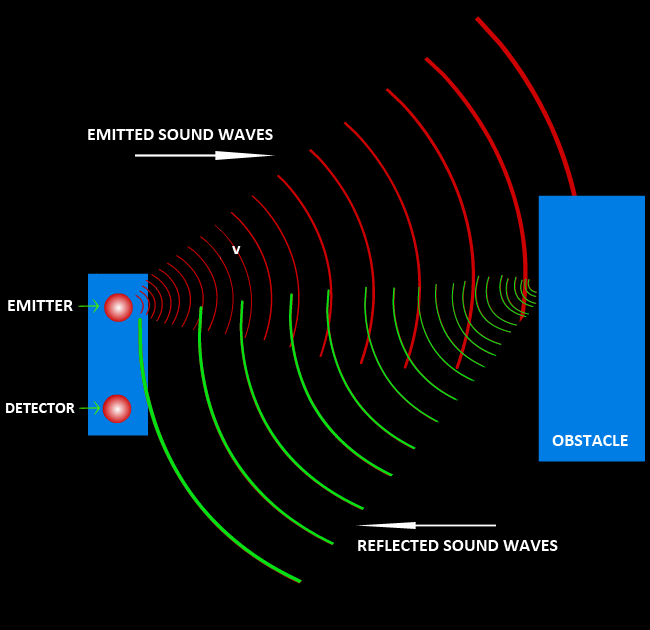
\includegraphics[scale=0.4]{CH02_Ultrasonic.png}
        \caption{Cara kerja sensor ultrasonik\cite{bs2}.}
        \label{fig:Ch02_ultrasonik}
    \end{figure}
    Seperti yang terlihat pada Gambar \ref{fig:Ch02_ultrasonik}, \textit{emitter} pada sensor ini akan memancarkan gelombang dan \textit{detector} akan menangkap gelombang pantul. Gelombang suara ultrasonik yang dikeluarkan adalah getaran pada frekuensi di atas jangkauan pendengaran manusia (\>20kHz) yang dapat merambat melalui berbagai media (udara atau cairan).

    Untuk menghitung jarak antara sensor dan objek, sensor mengukur waktu yang diperlukan antara pengeluaran gelombang oleh pemancar hingga kontaknya dengan penerima. Rumus untuk perhitungan ini adalah 
    \begin{equation}
        D = \frac{1}{2}T * C 
    \end{equation}
    \begin{tabbing}
        dengan : \= \\
        \>D : jarak,\\
        \>T : waktu,\\
        \>C : kecepatan suara (343 meter/detik dalam tekanan standar udara dan suhu 20° C).
    \end{tabbing}

    Sensor ultrasonik digunakan sebagai sensor jarak. Sensor ini dapat ditemukan dalam teknologi parkir mobil otomatis dan sistem keamanan anti-tabrakan. Sensor ultrasonik juga digunakan dalam sistem deteksi rintangan robot, serta teknologi manufaktur. Sensor ultrasonik tidak rentan dibandingkan dengan sensor inframerah (IR) dalam aplikasi pengindraan jarak terhadap gangguan asap, gas, dan partikel udara lainnya (meskipun komponen fisik masih dipengaruhi oleh variabel seperti panas).

    \subsection{Sensor Inframerah}
    \label{subsec:Infrared}

    \begin{figure}[H]
        \centering
        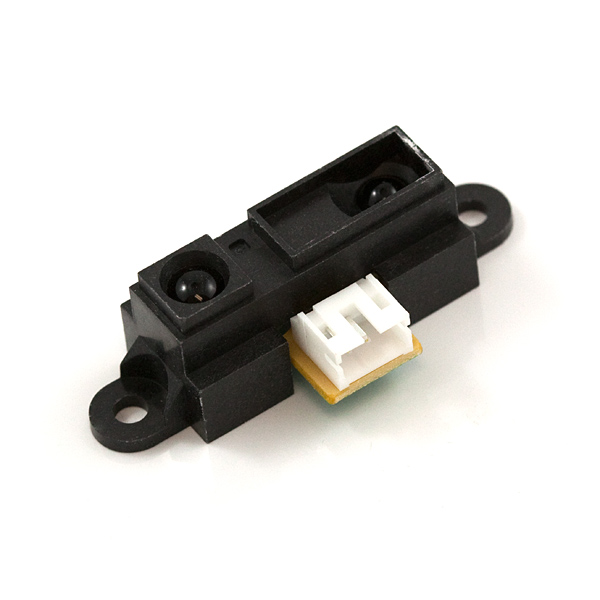
\includegraphics[scale=0.3]{infrared_sensor.jpg}
        \caption{Sensor Jarak Inframerah\cite{bs3}.}
        \label{fig:Ch02_inframerah}
    \end{figure}

    Sensor inframerah (sensor IR) adalah komponen \textit{optoelectronic} yang sensitif terhadap radiasi dengan sensitivitas spektrum dalam rentang panjang gelombang inframerah \SI{780}{\nano\metre} hingga \SI{50}{\micro\metre}\cite{bs4}. 
    Sensor yang terlihat pada Gambar \ref{fig:Ch02_inframerah} tersebut banyak digunakan sebagai detektor gerakan misalnya dalam gedung untuk menyalakan lampu atau dalam sistem alarm untuk mendeteksi penyusup. Sensor mendeteksi radiasi panas (radiasi inframerah) yang berubah seiring waktu dan ruang karena adanya pergerakan. Sensor ini juga banyak digunakan dalam perangkat peringatan gas, penganalisis gas, teknologi pengukuran gas medis, detektor api, dan pengukuran suhu presisi tanpa kontak. 

    Ada dua jenis sensor inframerah yaitu aktif dan pasif\cite{bs5}. Sensor inframerah aktif memancarkan dan mendeteksi radiasi inframerah. Sensor IR aktif memiliki dua bagian yaitu \textit{light-emitting diode} (LED) dan penerima. Objek yang mendekati sensor akan membuat cahaya inframerah dari LED memantul dari objek dan dideteksi oleh penerima. Sensor IR aktif bertindak sebagai sensor jarak, dan biasanya digunakan dalam sistem deteksi rintangan (seperti pada robot). Sensor inframerah pasif (PIR) hanya mendeteksi radiasi inframerah dan tidak memancarkannya dari LED.
    % https://www.researchgate.net/publication/261346136_Application_of_Infrared_sensor_for_shape_detection

    Sensor IR biasanya khusus dibuat sebagai sensor pengukur jarak tipe luaran analog yang terdiri dari light emitting diode (LED) dan detektor (photo-transistor), namun saat ini juga ada sensor IR yang memiliki tipe luaran digital. Konversi analog ke digital dengan tegangan 5 V dapat dihitung dengan persamaan:
    \begin{equation}
        \label{eqs: konversi_IR}
        jarak\ (cm)= \frac{2076}{luaran_{analog}-11}\cite{bs5}.
    \end{equation}
    Pengukuran jarak untuk sensor ini dibatasi hingga $30$ cm dan untuk meminimalkan tingkat \textit{noise} selama pengumpulan data. Pengukuran dengan cahaya inframerah dapat terganggu oleh sumber cahaya apa pun sehingga perlu diatur beberapa kondisi lingkungan selama pengambilan data seperti menggunakan sensor ini terbatas hanya pada ruangan yang dekat dan di tempat gelap\cite{bs6}.
    % K. Saman, "Twin Low-cost Infrared Range Finders for Detecting Obstacles Using in Mobile Platforms", in International Conference on Robotics and Biomimetics, Guangzhou, China, 2012, pp. 1996-1999.


    \subsection{Sensor \lidar\ (\textit{Light Detection and Ranging})}
    \label{subsec:lidar_sensor}
    
    \lidar\ (juga disebut LADAR) merupakan sensor optik yang digunakan untuk mengukur jarak dengan cara menembakkan cahaya ke target kemudian menangkap pulsa cahaya tersebut untuk dihitung jaraknya.  \lidar\ menggunakan sinar ultraviolet, cahaya tampak, atau inframerah agar dapat mendeteksi berbagai jenis target termasuk benda non-logam, batuan, hujan, dan senyawa kimia lainnya. Sinar laser dapat digunakan untuk memetakan fitur fisik dengan resolusi yang sangat tinggi. Saat ini \lidar\ dimanfaatkan untuk berbagai keperluan seperti mengukur jarak, menghitung kecepatan target bergerak, membaca lingkungan, mengestimasi lokasi target dan lain sebagainya. \lidar\ memiliki beberapa jenis antara lain yaitu \lidar\ 1D, \lidar\ 2D, dan \lidar\ 3D. Hal yang membedakan ketiganya adalah jumlah dimensi hasil bacaan. Pada Gambar \ref{fig:Ch02_3d_bacaan} terlihat hasil bacaan \lidar\ 3D yang memiliki 3 sumbu X,Y, dan Z.
    \begin{figure}[H]
        \centering
        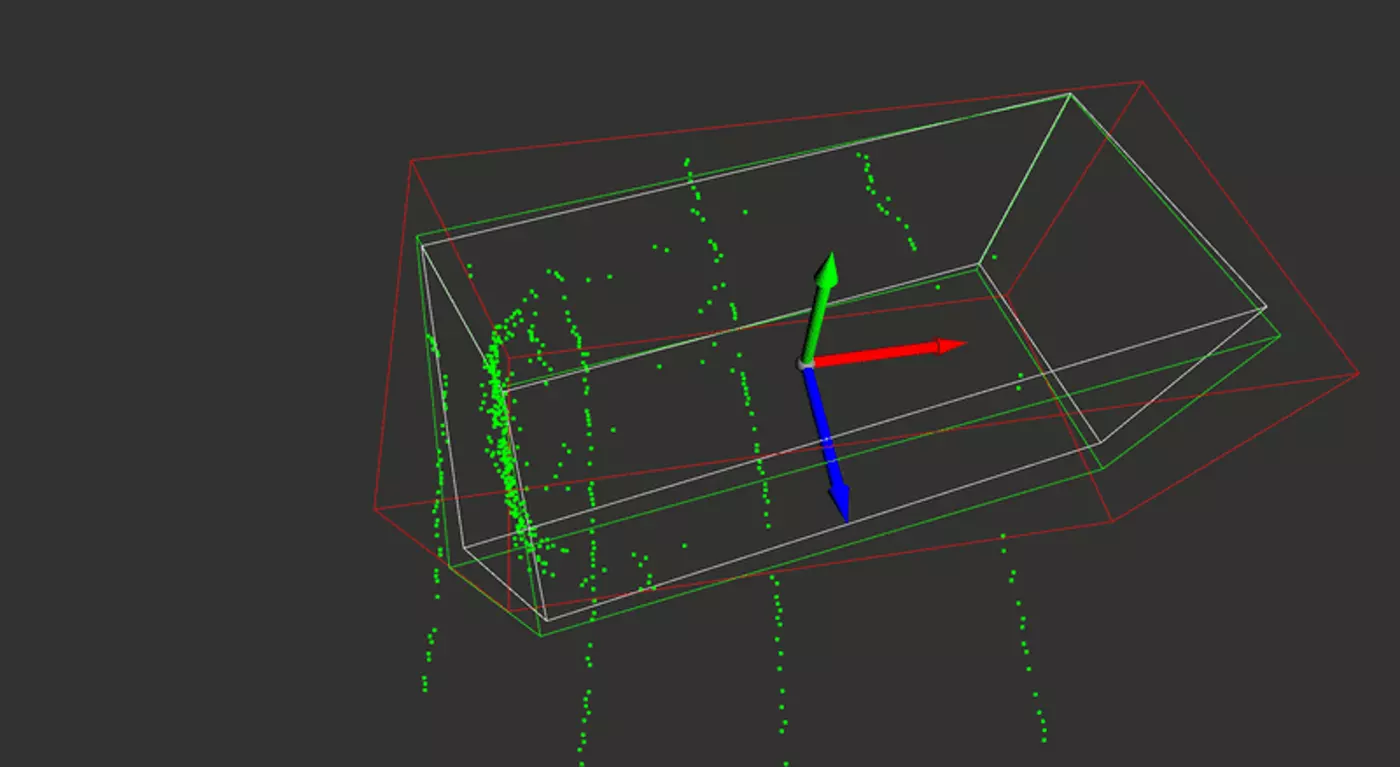
\includegraphics[scale=0.3]{3D_lidar_scanan.png}
        \caption{Contoh hasil bacaan \lidar\ 3D\cite{bs7}.}
        % https://understand.ai/blog/annotation/machine-learning/autonomous-driving/2021/03/29/3D-vs-2D-sensor-data-for-machine-perception.html
        \label{fig:Ch02_3d_bacaan}
    \end{figure}

    

    Tidak seperti kamera, \lidar\ berfungsi secara independen dari pencahayaan sekitar sehingga dapat memperoleh hasil yang baik saat siang dan malam tanpa kehilangan performa akibat gangguan seperti bayangan, sinar matahari, atau silau cahaya lampu \cite{bs8}.
    \begin{figure}[H]
        \centering
        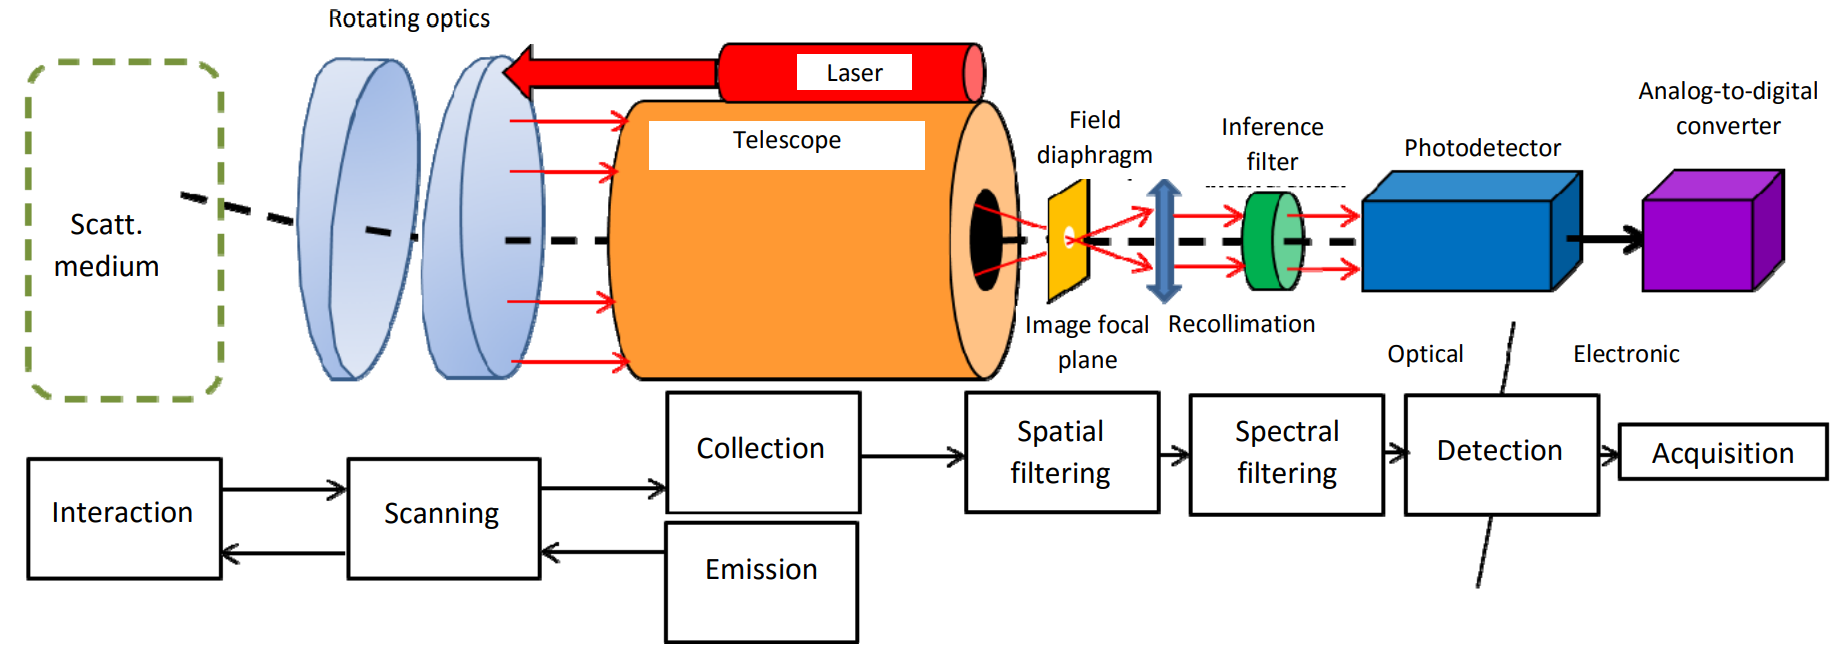
\includegraphics[width=\textwidth]{lidar_struktur.png}
        \caption{Gambar arsitektur \lidar\ Konvensional dan Fungsinya\cite{bs9}.}
        \label{fig:Ch02_lidar_struktur}
    \end{figure}
    % https://www.sciencedirect.com/science/article/pii/B9781785481024500053
    % See discussions, stats, and author profiles for this publication at: https://www.researchgate.net/publication/308941555
    Gambar \ref*{fig:Ch02_lidar_struktur} menunjukkan elemen-elemen penyusun \lidar\ konvensional beserta diagram fungsinya.
    Pulsa dipancarkan oleh sumber laser untuk setiap pengukuran LiDAR. Sinar laser yang dibentuk (diperluas dan dikoleksi) kemudian melewati optik pemindaian dan bergerak menuju media hamburan yang ditargetkan. Sinar yang mencapai target kemudian dihamburkan kembali ke arah LiDAR. Fluks optik dikumpulkan oleh sistem pencitraan optik, sering kali berdimensi besar seperti teleskop. 
    % A pulse is emitted by the laser source for each LiDAR measurement. Once the laser beam has been shaped (expanded and collimated), it passes through scanning optics and travels through space toward the targeted scattering medium. Following its interaction with the target, an echo of this pulse is backscattered toward the LiDAR. The optical flux is collected by an optical imaging system, often of large dimensions, such as a telescope. 
    \textit{Stray flux} dipisahkan dari sinyal melalui penyaringan spasial pada bidang fokus gambar juga melalui penyaringan spektral. Proses pertama membatasi bidang pandang ke ruang yang dilalui oleh pulsa laser, sedangkan yang terakhir digunakan untuk mengurangi bandwidth spektral sistem optik di sekitar panjang gelombang yang dipancarkan. Pemilihan panjang gelombang mengharuskan sinar untuk dikoleksi (paralel) di hulu elemen optik penyaringan spektral. Pada akhir rantai optik, fotodetektor mengubah aliran foton yang terdeteksi menjadi sinyal listrik kemudian  didigitalkan sebelum perekaman dan pemrosesannya. Penjelasan lebih lengkap mengenai bagian-bagian \lidar\ akan dijelaskan pada subbab \ref*{subsec: emisi} hingga subbab \ref*{subsec: Detection}.
    % Stray flux is separated from the signal by means of spatial filtering in the image focal plane as well as spectral filtering. The former restricts the field of view to the space traveled by the laser pulse, whereas the latter is used to reduce the spectral bandwidth of the optical system around the emitted wavelength. Note that wavelength selection requires the beam to be collimated (parallel) upstream of the spectral filtering optical element. At the end of the optical chain, a photodetector converts the detected photon flow into an electrical signal, which is in turn digitized prior to its recording and processing.
    \subsubsection{Emisi \lidar}
    \label{subsec: emisi}
    Transmisi berasal dari sumber pulsa laser yang memancarkan inframerah dekat (panjang gelombang 780-3.000 nm), terlihat (390-780 nm) atau domain ultraviolet (200-390 nm). Berbagai macam sumber laser dipasang di sekitar media penguat yang dapat berupa sel gas, kristal, dioda atau serat. Pemilihan panjang gelombang yang dipancarkan untuk aplikasi kehutanan dikondisikan berdasarkan transmisi atmosfer dan reflektansi vegetasi. Persyaratan lain dalam hal kekompakan, stabilitas, dan energi yang dipancarkan juga harus dipertimbangkan terutama dalam kasus durasi pulsa dari urutan beberapa nanodetik (diperlukan dalam kasus resolusi vertikal lebih rendah dari 1 m) dan frekuensi pengulangan yang tinggi.
    % The transmission is derived from a pulsed laser source emitting in the near-infrared (IR, wavelength 780-3,000 nm), visible (390-780 nm) or near- ultraviolet domain (UV, 200-390 nm). A wide variety of laser sources are built around amplifying media which can be gas cells, crystals, diodes or fibers. In the case of space or airborne LiDARs for forestry applications, the selection of the emitted wavelength is conditioned by atmospheric transmission and vegetation reflectance. Other requirements in terms of compactness, stability and emitted energy must also be taken into  consideration, especially in the case of pulse durations of the order of a few nanoseconds (required in the case of a vertical resolution lower than 1 m), and high repetition frequency. These various constraints restrict the selection to a range of basic sources summarized in Table 5.3. The table is ordered by the type of solid amplifying medium used.
    Dioda laser merupakan sumber laser yang paling kuat dan kompak yang dapat ditemukan dalam mode pulsa di dekat media IR. Panjang gelombang yang paling umum digunakan dan menguntungkan dalam hal energi adalah 905 nm. Dioda ini telah menjadi fitur jangkauan laser dan kontrol kecepatan pada \lidar, namun energi terbatas dioda membuat jangkauan LiDAR terbatas hingga beberapa ratus meter saja.
    % Laser diodes, the most robust and compact laser sources, may be found in pulsed mode in the near IR medium. The most commonly used and favorable wavelength in terms of energy is 905 nm. These diodes have become a feature of laser range-finders and speed control LiDARs. However, their energy remains limited (a few microjoules), which restricts the range of the LiDAR to a few hundred meters. Also in the near IR domain, fiber lasers at 1,064 nm (ytterbium) and 1,550 nm (erbium) are sufficiently compact and emit energy pulses of a few hundred microjoules.

    % 5.3.2.2. Transmitted beam shaping
    Sinar pada output laser biasanya harus sedikit menyebar dan diameternya meningkat untuk memenuhi kriteria yang berkaitan dengan keamanan mata. Divergensi sinar juga disesuaikan sesuai metode pengukuran yang dipilih, misalnya jejak kecil ( cm) dalam kasus gema diskrit \lidar\ atau pemindaian \lidar\ atau jejak besar dalam kasus \lidar\ gelombang penuh. Terdapat sistem optik \textit{afocal} yang melakukan pembentukan sinar terdiri dari dua lensa atau cermin yang menggabungkan titik fokus sedemikinan sehingga pembesaran yang dihasilkan lebih tinggi dari 1, seperti yang ditunjukkan pada Gambar \ref*{fig:Ch02_lidar_emisi}.
    \begin{figure}[H]
        \centering
        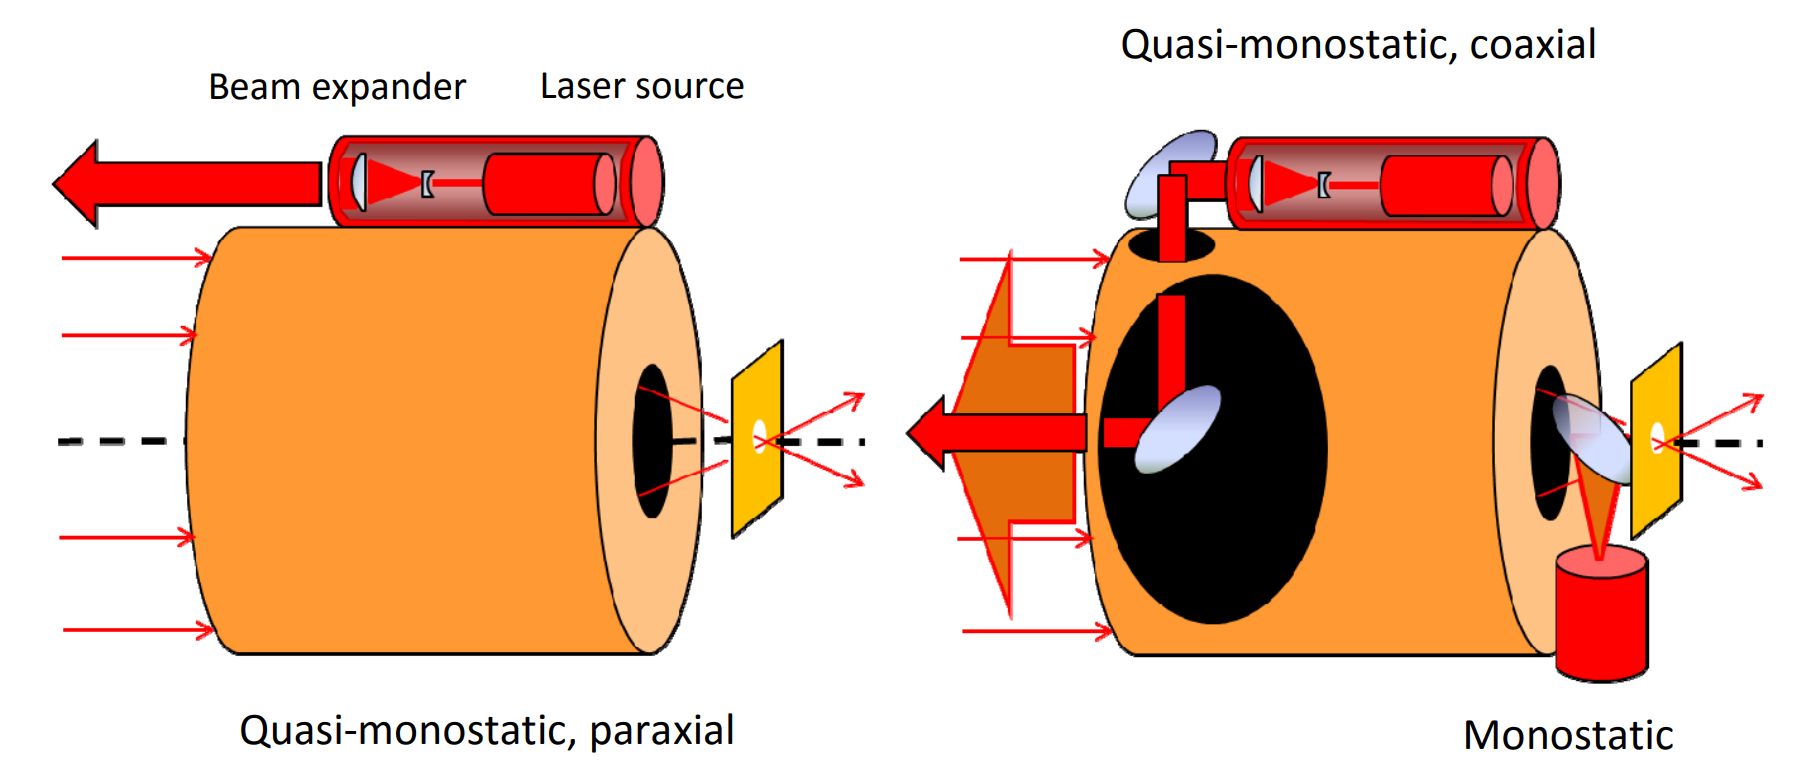
\includegraphics[width=0.7\textwidth]{emisi_lidar.png}
        \caption{Contoh Konfigurasi Emisi \lidar\cite{bs9}.}
        \label{fig:Ch02_lidar_emisi}
    \end{figure}
    
    Konfigurasi \lidar\ ditentukan oleh tata letak jalur pemancar dan penerimaan seperti yang disajikan pada Gambar \ref*{fig:Ch02_lidar_emisi}. Kedua komponen sistem optronik jika memiliki sumbu optik yang sama maka sistem tersebut dinamakan sebagai \textit{“monostatic”} sedangkan jika sumbu berbeda dan terpisah secara spasial maka disebut sebagai \textit{“bistatic”}. Konfigurasi terakhir juga memfasilitasi lewatnya jalur pemancar dan penerimaan melalui optik pemindaian yang sama.
    
    % A LiDAR configuration is determined by the layout of the emitting and receiving paths, as presented in Figure 5.4. If the two components of an optronic system have the same optical axis, said system is referred to as “monostatic”, whereas if the axes are distinct and spatially separated, it is referred to as “bistatic”. In our case, the proximity between the emitter and the receiver results in the LiDAR sensor being referred to as a “quasimonostatic” system, which represents an intermediate case. Systems in surface applications can adopt the so-called paraxial configuration, shown on the right. Nevertheless, in order to allow the overlap of emission and reception over a greater distance, a coaxial or fully monostatic configuration can be preferred, shown on the left. The latter configuration also facilitates the passage of the emitting and receiving paths through the same scanning optics.
% At the laser output, the beam usually has to be slightly divergent and its diameter increased, in order to meet the criteria pertaining to eye safety. If the laser beam is not eye-safe at emission, the aim is to reduce the nominal ocular hazard distance (NOHD) below the flight altitude or values provided by aviation specifications (a few hundred meters). Beam divergence is also adjusted as a function of the measuring method selected: a small footprint (~cm) in the case of a discrete echo LiDAR or a scanning LiDAR, or a large footprint in the case of a full waveform LiDAR. An afocal optical system carries out the beam shaping. It is made up of two lenses or mirrors having merged focal points and a resulting magnification higher than 1, as shown in Figure 5.4.

\subsubsection{Pemindaian}
\label{subsec: Scanning}
    \begin{figure}[H]
        \centering
        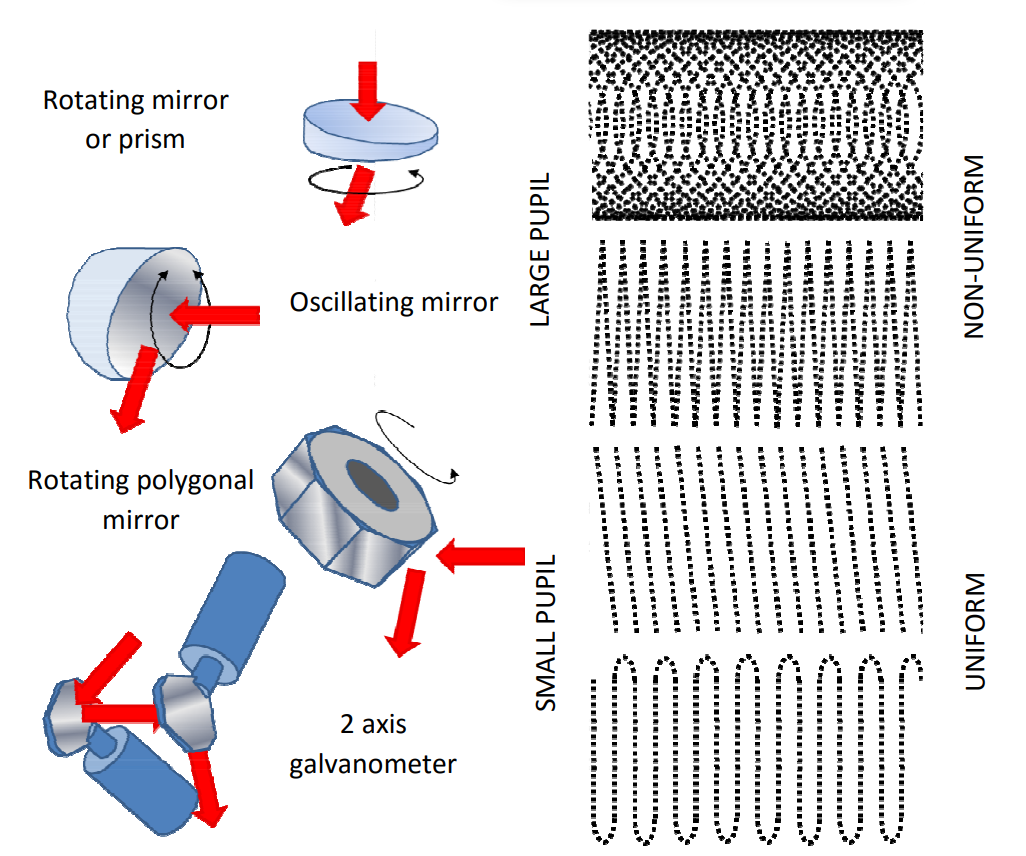
\includegraphics[scale=0.3]{pemindaian_lidar.png}
        \caption{Jenis-jenis Alat Pemindaian \lidar\ dan Pola Pemindaiannya\cite{bs9}.}
        \label{fig:Ch02_pemindaian_lidar}
    \end{figure}

    Berbagai elemen optik digunakan untuk menerapkan sistem \lidar\ yang mampu dengan cepat mengambil sampel pada permukaan besar. Empat solusi beserta pola pemindaian yang dihasilkan diilustrasikan pada Gambar \ref*{fig:Ch02_pemindaian_lidar}. Terlihat bahwa posisi berurutan jejak kaki laser pada jalur ini dikondisikan oleh frekuensi pengulangan pulsa. Pola-pola ini memiliki arti bahwa pengambilan sampel yang didistribusikan secara seragam tidak dapat dicapai dengan menggunakan optik berputar biasa. 
    Masalah lainnya yang terkait dengan implementasi sistem pemindaian adalah bahwa elemen terakhir harus mengakomodasi jalur pemancar dan penerimaan dengan minimal \textit{cross-talk}. Namun, sistem tercepat yang mampu menyediakan pemindaian seragam harus memiliki pupil kecil. Hal ini mengurangi dimensi sensor dan juga membatasi tingkat daya yang diterima.
% Various mobile optical elements may be used in order to implement an airborne scanning LiDAR system capable of quickly sampling large surfaces. Four such solutions are illustrated in Figure 5.5, along with the associated scanning patterns. It is clear that the consecutive positions of laser footprints on these paths are conditioned by the pulse repetition frequency (see section 5.3.2.1). It can still be inferred from these patterns that a uniformly distributed sampling cannot be achieved using basic rotating optics. Another severe constraint associated with the implementation of a scanning system is that the latter has to accommodate both emitting and receiving paths, with a minimum of cross-talk. However, the fastest systems capable of providing uniform scanning have small pupils. This imposes reduced sensor dimensions and therefore restricts the levels of power received.

\subsubsection{Penerimaan Fluks}
\label{subsec: receiving}

Berbagai macam sistem optik untuk menerima \textit{backscattered flux} dikembangkan sesuai dengan aplikasinya. Contoh lensa optik yang digunakan untuk menerima fluks yaitu:
\begin{enumerate}
    \item  Sistem \textit{catoptric} dan \textit{catadioptric}, termasuk cermin dan lebih sering disebut sebagai teleskop reflektif. Sistem ini berdiameter besar dan tidak mengalami aberasi kromatik yang mengurangi resolusi ketika pengamatan dilakukan pada spektrum yang luas. 
    % catoptric and catadioptric systems include mirrors and are more commonly referred to as reflective telescopes. These are large diameter systems that do not suffer from chromatic aberration, which reduces resolution when observations are conducted over a wide spectrum. 
    \item Sistem dioptrik (teleskop bias atau refraktor), hanya terdiri dari lensa dan jarang memiliki diameter yang sama dengan teleskop reflektif tanpa biaya tambahan atau berat dan dimensi keseluruhan yang kecil. Pada kasus \lidar\ monokromatik dan nilai diameter yang wajar, sistem ini masih dapat memberikan peningkatan kekompakan dan \textit{throughput}. Keuntungan utama sistem ini adalah stabilitasnya yang tinggi terhadap getaran yang memfasilitasi implementasinya pada \textit{platform} udara.
    % dioptric systems (refractive telescopes or refractors), solely made up of lenses, can rarely have the same diameter as reflective telescopes without additional costs or an inadmissible weight and overall dimensions. In the case of monochromatic LiDARs and reasonable diameter values, these systems can still provide improved compactness and throughput. Another major advantage is their high stability against vibrations, which facilitates their implementation on an airborne platform.
\end{enumerate}

Setelah fluks cahaya dikumpulkan, fluks dapat disuntikkan ke dalam serat optik yang ditempatkan di titik fokus sistem penerimaan untuk memisahkan deteksi dari kepala optik \lidar. Hal ini juga memungkinkan untuk membatasi obstruksi teleskop dengan menempatkan serat pada fokus cermin utama atau menggabungkan aliran beberapa teleskop sehingga menghasilkan pengurangan biaya dibandingkan dengan menggunakan satu teleskop besar. Serat optik terdiri dari inti dan dilapisi silika dengan indeks bias yang sedikit berbeda yang memungkinkan lewatnya cahaya. Diameternya harus dibatasi menjadi beberapa ratus mikron untuk menjaga fleksibilitas.
% Once the light flux has been collected, it can be injected into an optical fiber placed in the focal point of the reception system in order to dissociate the detection from the optical head of the LiDAR. This also makes it possible to limit telescope obstruction by placing the fiber at the focus of the primary mirror, or to combine the flow of several telescopes, a solution which results in reduced costs compared to a single larger telescope. An optical fiber is made up of a core and clad made of silica with slightly different refractive indices, which allows the assembly to guide light. Its diameter is limited to a few hundred microns in order to maintain flexibility.
% If used, it becomes the field diaphragm of the reception system, and reduces the field of view of the LiDAR to a great extent. The field of view can be expanded by using a bundle of fibers and a field lens, but this generates insertion losses which can amount to up to 60% of the incident light. 
% In the case of a good quality optical system, well adjusted in terms of focal length, the only dimensioning parameters of the receiver are its field of view and its effective area Aer which is connected to its actual area A and expressed as:

\subsubsection{\textit{Filtering}}
\label{subsec: Filtering}
Tingginya luminans lingkungan pada siang hari disebabkan ultraviolet atau inframerah menyebabkan perlunya untuk menyaring fluks cahaya yang masuk baik secara spasial maupun spektral. Proses ini diilustrasikan pada Gambar \ref*{fig:Ch02_filter_lidar}. Gambar menunjukkan proses penyaringan fluks yang datang untuk bidang fokus dan pupil.
\begin{figure}[H]
    \centering
    \begin{subfigure}[b]{.40\textwidth}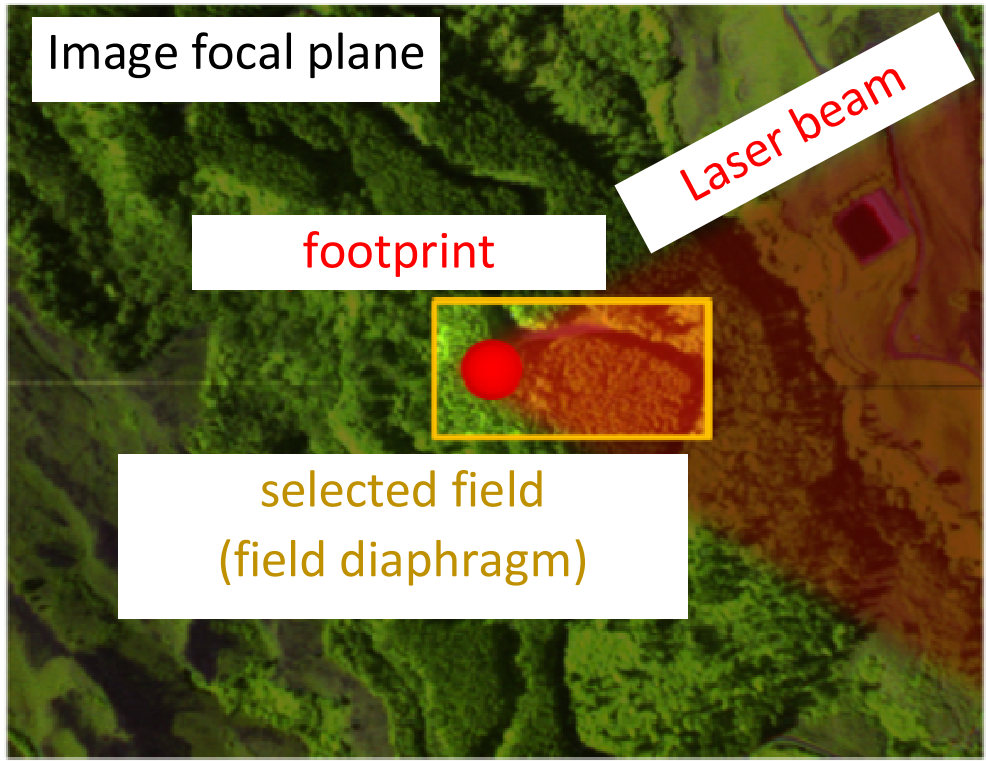
\includegraphics[width=\linewidth]{lidar_filtering.png}\caption{\textit{Spatial Filtering}}\label{Fig:Ch02_lidar_filtering1}\end{subfigure}
    \begin{subfigure}[b]{.40\textwidth}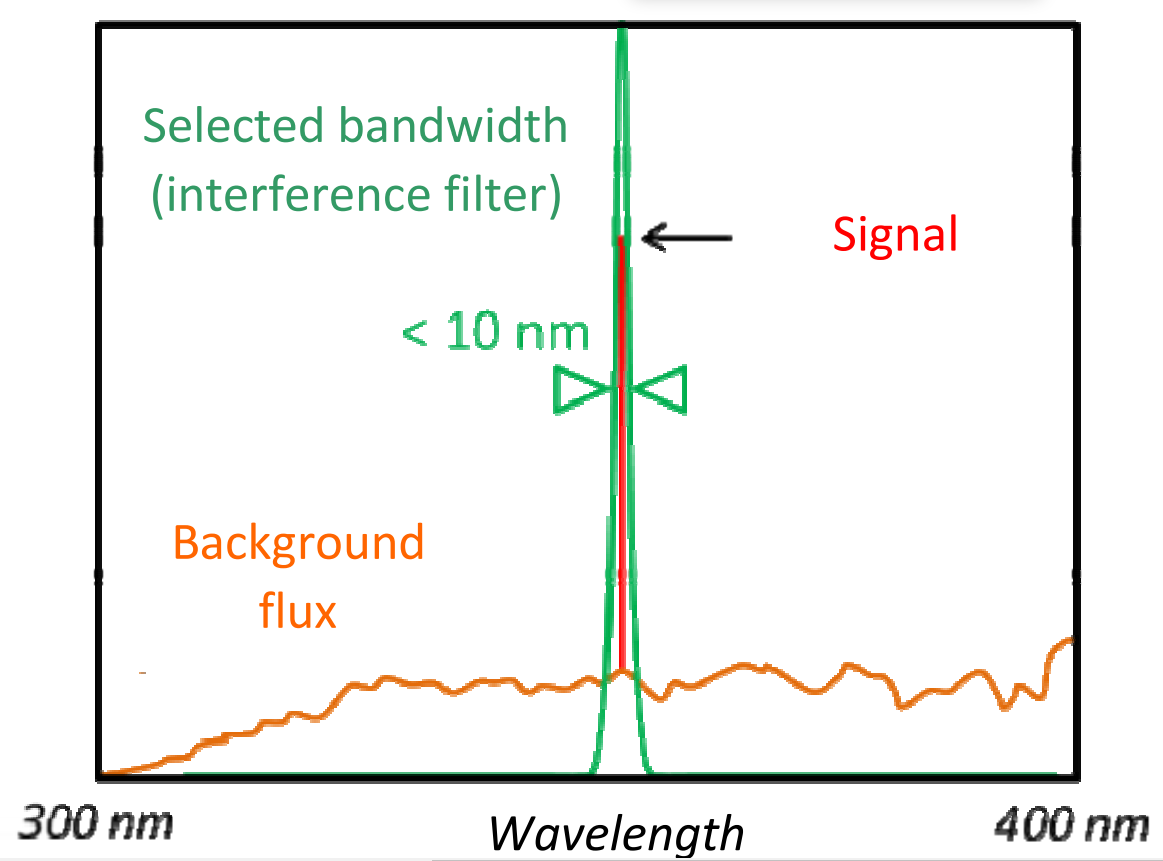
\includegraphics[width=\linewidth]{lidar_filtering2.png}\caption{\textit{Spectral Filtering}}\label{Fig:Ch02_lidar_filtering2}\end{subfigure}
    \caption{Proses Penyaringan Fluks Cahaya pada \lidar\cite{bs9}.}
    \label{fig:Ch02_filter_lidar}
\end{figure}
Pada bidang fokus gambar, diafragma lapangan membatasi bidang pandang sistem secara tepat ke ruang yang dilalui oleh sinar laser. Diafragma medan yang optimal untuk kasus konfigurasi paraksial adalah persegi panjang seperti yang diwakili pada Gambar 5.6. Konsekuensi dari keterbatasan bidang ini adalah adanya jarak pengukuran yang minimum, dalam kasus konfigurasi non-monostatik maka sinar hanya dapat memasuki bidang secara progresif.
% Due to the high luminance of daytime environment from near-ultraviolet o near-infrared, it is necessary to filter the incoming light flux both in a spatial and a spectral manner. This process is illustrated in Figure 5.7. In the image focal plane, a field diaphragm restricts the field of view of the system precisely to the space traveled by the laser beam. The optimum field diaphragm is rectangular in the case of a paraxial configuration, as represented in Figure 5.6. A consequence of this limitation of the field is the existence of a minimum measurement distance, knowing that: - in the case of non-monostatic configurations, the beam can only enter the field in a progressive manner;
Pada bidang pupil (misalnya pada sinar yang dikoleksi ulang setelah fokus pertama), ditempatkan filter dengan kemampuan spektral yang tinggi dan berpusat pada panjang gelombang yang dipancarkan untuk secara signifikan mengurangi \textit{bandwidth} sistem \lidar. Lebar spektral emisi kurang dari nanometer kecuali dalam kasus dioda laser dengan filter interferensi yang ditandai dengan lebar mulai dari 0,5 hingga 10 nm dapat digunakan. Komponen optik semacam itu dibangun menggunakan tumpukan film tipis dari tipe Bragg dan Fabry–Pérot untuk memadamkan spektrum yang luas dan membiarkan melalui garis sempit. 
% In the pupil plane (for example, on a recollimated beam after the first focus), a filter with a great spectral finesse and centered at the emitted wavelength is placed, in order to significantly reduce the bandwidth of the LiDAR system. The spectral width of the emission being less than a nanometer except in the case of laser diodes, an interference filter characterized by a width ranging from 0.5 to 10 nm can be used. Such an optical component is built using thin film stacks of the Bragg and Fabry–Pérot type in order to quench a broad spectrum and let through a narrow line. 

\subsubsection{Konversi Fluks ke Tegangan}
\label{subsec: Detection}
Konversi sinyal fluks optik menjadi tegangan listrik yang dapat diukur dilakukan oleh fotodetektor dengan mengubah setiap foton menjadi fotoelektron (dengan probabilitas yang ditetapkan oleh efisiensi kuantumnya) yang dilepaskan dalam resistor beban. Detektor cepat dan sangat sensitif yang digunakan dalam \lidar\ menyediakan sejumlah besar fotoelektron (antara 10 dan 10.000) untuk setiap foton insiden melalui fenomena penguatan internal. Kedua jenis detektor ini memiliki karakteristik yang sangat berbeda dalam hal sensitivitas, \textit{noise}, atau kapasitas listrik. Berbagai fenomena ini memiliki dampak signifikan pada \textit{link budget}, khususnya sebagai fungsi dari panjang gelombang yang dipilih untuk \lidar. 
% The conversion of the optical flux signal into measurable electric voltage is performed by a photodetector, which transforms each photon into a photoelectron (with a probability fixed by its quantum efficiency) discharged in a load resistor. The fast and highly sensitive detectors used in LiDAR, whether avalanche photodiodes (near IR) or photomultipliers (visible and UV), provide a large number of photoelectrons (between 10 and 10,000) for each incident photon via an internal gain phenomenon. Nevertheless, these two types of detectors have very different characteristics in terms of sensitivity, noise or electrical capacity (the latter restricting temporal resolution). These various phenomena have a significant impact on the link budget, in particular as a function of the wavelength selected for the LiDAR. The electronic detection configurations and the spectral ranges of various LiDAR detectors are illustrated in Figure 5.8. Table 5.5 presents the characteristics of these various internal gain photodetectors and more conventional photodiodes. They can be used in analog and photon counting mode.

% Robot Operating System
\section{Sistem Operasi Robot}
\label{sec:ROS} 

    Berbagai sistem operasi untuk robot saat ini telah dikembangkan. Sistem-sistem ini dapat digunakan untuk memprogram dan menyimulasikan robot dengan lebih mudah.
    Sebelum ada pengembangan sistem operasi robot, setiap \dev\ membuat program dari awal yang biasanya tidak bisa langsung diaplikasikan dan dikembangkan ke dalam robot lain.
    Berbagai sistem operasi dan program muncul untuk menjadi platform umum pada pengembangan aplikasi robotika. Berbagai sistem dapat digunakan untuk tujuan komersial maupun penelitian secara gratis dan \textit{open source}. Adanya algoritma siap pakai yang sudah tersedia dan dukungan komunitas yang besar membuat pengembangannya lebih mudah.
    
    \textit{Robot Operating System} (ROS) merupakan salah satu perangkat lunak khusus pengembangan robot yang bersifat \textit{open source} dengan \textit{libraries} dan \textit{tools} yang sudah tersedia untuk membangun program pada robot. ROS memiliki fitur yang banyak. Biasanya \dev\ menggunakan ROS untuk membuat prototipe, ROS tidak digunakan untuk membuat produk sebenarnya dikarenakan berbagai alasan seperti keamanan dan kekurangan pada pemrosesan \textit{real-time}\cite{br1}. Beberapa fitur ROS yang mendukung pengembangan robot antara lain yaitu:
    \begin{itemize}
     \item ROS menyediakan antarmuka penyampaian pesan untuk komunikasi antara dua program atau proses.
     \item ROS bukanlah sistem operasi yang sebenarnya tetapi merupakan sistem operasi meta yang menyediakan beberapa fungsi dan fitur mirip sistem operasi asli.
     \item ROS Mendukung bahasa pemrograman tingkat tinggi dan berbagai \textit{tools}.
     \item Kerangka kerja ROS terintegrasi dengan berbagai \textit{libraries} yang populer seperti OpenCV dan PCL.
     \item Algoritma siap pakai.
     \item ROS mudah digunakan untuk pembuatan prototipe.
     \item Komunitas pengembang yang banyak.
     \item \textit{Tools} dan simulator yang luas.
     \end{itemize}
% Why use ros?
% This is common question that developers ask when looking for a platform to program ROS. Although ROS has many features, there are still areas in which ROS can’t be used or is not recommended to use. In the case of a self-driving car, for example, we can use ROS to make a prototype, but developers do not recommend ROS to make the actual product. This is due to various issues, such as security, real-time processing, and so forth. ROS may not be a good fit in some areas, but in other areas, ROS is an absolute fit. In corporate robotics research centers and at universities, ROS is an ideal choice for prototyping. And ROS is used in some robotics products after lot of fine-tuning (but not self-driving cars).
% There was active development in robotics before the ROS project, but there was no common platform and community for developing robotics applications. Each developer created software for their own robot, which in most cases, couldn’t be reused for any other robot. Developers had to rewrite code from scratch for each robot, which takes a lot of time. Also, 
% most of the code was not actively maintained, so there was no support for 
% the software. Also, developers needed to implement standard algorithms 
% on their own, which took more time to prototype the robot.
% After the ROS project, things changed. Now there is a common platform for developing robotics applications. It is free and open source for commercial and research purposes. Off-the-shelf algorithms are readily available, so there is no longer a need to code. There is big community support, which makes development easier. In short, the ROS project changed the face of robotics programming.

\section{\textit{Object Recognition}}
\label{sec:object_detection} 

\textit{Object recognition} adalah bentuk aplikasi dasar untuk pemrosesan gambar dan visualisasi pada komputer. Istilah ini digunakan dalam berbagai aplikasi dan algoritma. Secara umum \objd\ bertujuan untuk mengingat data tentang penampilan objek tertentu dan memeriksa untuk mengevaluasi objek tersebut jenis apa dan di mana letaknya. 

\begin{figure}[H]
            \centering
            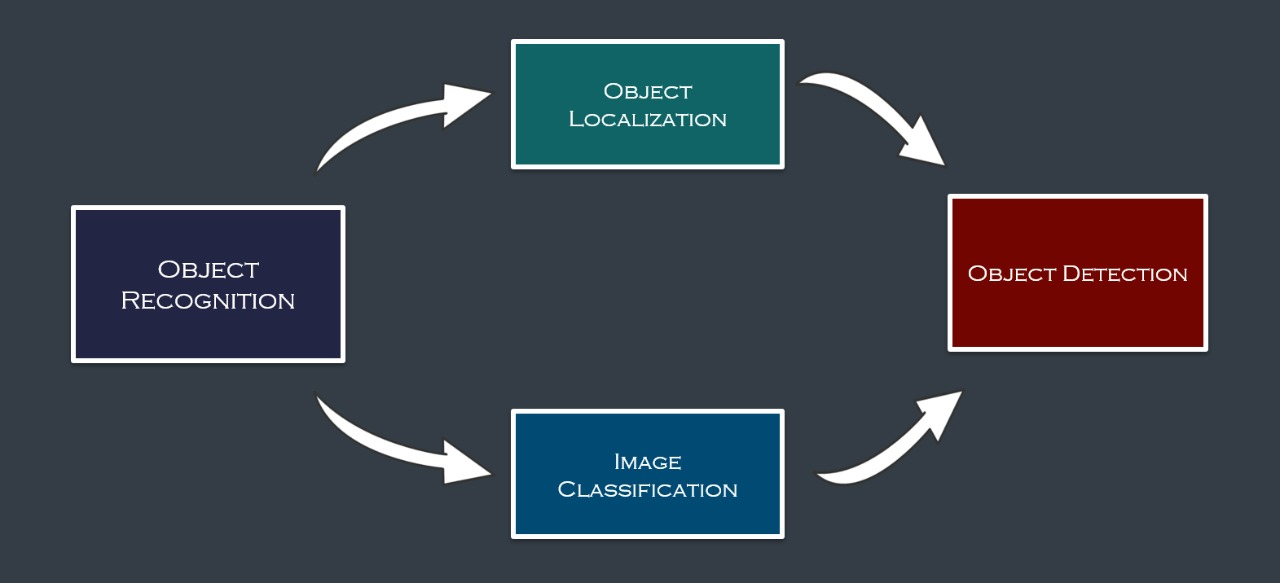
\includegraphics[scale=0.3]{Object_Rec.jpeg}
            \caption{Diagram Proses \textit{Object Recognition}.}
            \label{fig:Ch02_objectR}
        \end{figure}

Pada Gambar \ref{fig:Ch02_objectR} terlihat bahwa dalam object recognition terdapat dua proses terpisah yaitu \textit{object localization} dan \textit{image classification}. \textit{Object localization} merupakan komponen untuk menentukan posisi dan jarak benda atau objek yang terdeteksi di sekitar lingkungan. Image classification berfungsi untuk mengklasifikasi jenis objek yang terdeteksi. Kedua proses ini kemudian digabungkan menjadi \textit{object detection}. \textit{Object detection} biasanya menampilkan hasil klasifikasi dan letak objek hasil pemrosesan dalam \textit{bounding box} dengan keterangan nama objek. 

Ada banyak pendekatan yang berbeda untuk merancang \objd\, masing-masing memperhitungkan tuntutan spesifik dari konteks aplikasi yang diinginkan. Kategorisasi metode dan mode operasi dapat dikelompokkan melalui beberapa kriteria yang mengacu pada properti model data yang mewakili objek dan mode operasi skema \objd. Kriteria-kriteria tersebut adalah sebagai berikut\cite{br2}:
\begin{itemize}
\item Representasi objek yang diperoleh dengan mencari informasi tentang objek dapat diidentifikasi yaitu dengan geometri atau penampilan. Informasi geometris mengacu pada batas atau  bentuk permukaan objek. Sementara itu, model berbasis tampilan diturunkan dari karakteristik potret wilayah yang dicakup oleh objek.
\item Cakupan data objek yang dapat merujuk pada properti lokal objek (contoh: posisi sudut objek) atau karakteristik objek global (contoh: area, keliling, momen inersia).
\item Variasi objek yang dapat ditunjukkan oleh individu yang berbeda dari kelas objek yang sama.
\item Kualitas data gambar.
\item Strategi pencocokan untuk mengenali objek dalam gambar dilakukan di beberapa titik dalam aliran algoritma, misalnya pada model objek harus disejajarkan dengan konten gambar dengan cara kesamaan antara model dan gambar dimaksimalkan atau perbedaan diminimalkan.
\end{itemize}

%Sumber dari buku An Introduction to Object Recognition